
%
\RequirePackage{docswitch}
\setjournal{\flag}

\documentclass[\docopts]{\docclass}

% You could define the document class directly
%\documentclass[]{emulateapj}

% 
\usepackage{soul} 
\usepackage{amsmath}
\usepackage{xspace}
\usepackage{xifthen}
\usepackage[dvipsnames,svgnames]{xcolor} 

% General formatting
\newcommand{\ie}{i.e.\xspace}
\newcommand{\eg}{e.g.\xspace}
\newcommand{\etc}{etc.\xspace}
\newcommand{\etal}{et al.\xspace}
\newcommand{\vs}{vs.\xspace}
\newcommand{\super}[1]{\ensuremath{^{\textrm{#1}}}}
\newcommand{\sub}[1]{\ensuremath{_{\textrm{#1}}}}

\newcommand{\FIXME}[1]{{\bf \textcolor{red}{#1}}}
%\newcommand{\FIXME}[1]{{#1}}
\newcommand{\CHECK}[1]{{\bf \textcolor{orange}{#1}}}
%\newcommand{\CHECK}[1]{{#1}}
\newcommand{\COMMENT}[1]{{\it \textcolor{blue}{#1}}}
%\newcommand{\COMMENT}[1]{{#1}}
\newcommand{\NEW}[1]{{\textcolor{blue}{#1}}}
%\newcommand{\NEW}[1]{{#1}}

% Math
\mathchardef\mhyphen="2D
\newcommand{\vect}[1]{\boldsymbol{#1}}
\newcommand{\roughly}{\ensuremath{ {\sim}\,} }
\newcommand{\gtr}{\ensuremath{ {>}\,} }
\newcommand{\less}{\ensuremath{ {<}\,} }
\newlength{\dhatheight}
\newcommand{\doublehat}[1]{%
    \settoheight{\dhatheight}{\ensuremath{\hat{#1}}}%
    \addtolength{\dhatheight}{-0.35ex}%
    \hat{\vphantom{\rule{1pt}{\dhatheight}}%
    \smash{\hat{#1}}}}
\newcommand{\code}[1]{\texttt{#1}\xspace}
\newcommand{\dd}{\ensuremath{\rm d}}
\newcommand{\var}[1]{\ensuremath{#1}\xspace}


% Referencing 
\newcommand{\secref}[1]{Section~\ref{sec:#1}}
\newcommand{\appref}[1]{Appendix~\ref{app:#1}}
\newcommand{\tabref}[1]{Table~\ref{tab:#1}}
\newcommand{\tabrefs}[2]{Tables~\ref{tab:#1} and \ref{tab:#2}}
\newcommand{\figref}[1]{Figure~\ref{fig:#1}}
\newcommand{\figrefs}[2]{Figures~\ref{fig:#1} and \ref{fig:#2}}
\newcommand{\eqnref}[1]{Equation~\eqref{eqn:#1}}

% Astronomy
\newcommand{\LCDM}{\ensuremath{\rm \Lambda CDM}\xspace}
\newcommand{\ra}{{\ensuremath{\alpha_{2000}}}\xspace}
\newcommand{\dec}{{\ensuremath{\delta_{2000}}}\xspace}
\newcommand{\glon}{{\ensuremath{\ell}}\xspace}
\newcommand{\glat}{{\ensuremath{b}}\xspace}

% Units
\newcommand{\unit}[1]{\ensuremath{\mathrm{\,#1}}\xspace}
\newcommand{\Gyr}{\unit{Gyr}}
\newcommand{\MeV}{\unit{MeV}}
\newcommand{\GeV}{\unit{GeV}}
\newcommand{\TeV}{\unit{TeV}}
\newcommand{\degree}{\ensuremath{{}^{\circ}}\xspace}
\newcommand{\mas}{\unit{mas}}
\newcommand{\amin}{\unit{arcmin}}
\newcommand{\asec}{\unit{arcsec}}
\newcommand{\angstrom}{\unit{\AA}}
\newcommand{\um}{\unit{$\mu$m}}
\newcommand{\cm}{\unit{cm}}
\newcommand{\km}{\unit{km}}
\newcommand{\pc}{\unit{pc}}
\newcommand{\kpc}{\unit{kpc}}
\newcommand{\second}{\unit{s}}
\newcommand{\us}{\unit{$\mu$s}}
\newcommand{\photons}{\unit{ph}}
\newcommand{\photon}{\unit{ph}}
\newcommand{\sr}{\unit{sr}}
\newcommand{\Msolar}{\ensuremath{M_\odot}}
\newcommand{\Msun}{\ensuremath{M_\odot}}
\newcommand{\Mstar}{\ensuremath{M_{*}}}
\newcommand{\Lsolar}{\ensuremath{L_\odot}}
\newcommand{\Lsun}{\ensuremath{L_\odot}}
\newcommand{\Lstar}{\ensuremath{L_{*}}}
\newcommand{\Lum}{\ensuremath{ L }\xspace}
\newcommand{\cmcubes}{\ensuremath{\cm^{3}\second^{-1}}\xspace}
\newcommand{\magn}{\unit{mag}}
\newcommand{\mmag}{\unit{mmag}}
\providecommand{\deg}{}
\renewcommand{\deg}{\unit{deg}}
\newcommand{\kms}{{\km\second^{-1}}}
% 

\bibliographystyle{apj}

\usepackage[outdir=./]{epstopdf}
\usepackage{graphicx,verbatim}
\usepackage{xspace}
\usepackage[figuresright]{rotating}
\usepackage{tabularx}
\setlength{\rotFPtop}{0pt plus 3fil}
\setlength{\rotFPbot}{0pt plus 1fil}
\setlength{\rotFPtop}{0pt plus 1fil}

\graphicspath{{./}{./figures/}}
\newcommand{\nv}{\hat{\bf n}}
\newcommand{\todo}[1]{\textcolor{magenta}{To do: #1}}
\newcommand{\vol}[1]{\textcolor{red}{Volunteer(s) in charge: #1}}
\newcommand{\cont}[1]{\textcolor{blue}{Suggested content: #1}}
\newcommand{\mrm}[1]{\mathrm{#1}}
\newcommand{\sukhdeep}[1]{\textcolor{magenta}{SS: #1}}
\newcommand{\damonge}[1]{\textcolor{green!55!blue}{DA: #1}}
\newcommand{\asv}[1]{\textcolor{purple}{ASV: #1}}
\newcommand{\revise}{\textcolor{red!55!blue}{\bf Section ready for revision}}
\newcommand{\jab}[1]{\textcolor{blue}{JAB: #1}}
\newcommand{\mi}[1]{\textcolor{brown}{MI: #1}}
\newcommand{\tom}[1]{\textcolor{cyan}{TM: #1}}

\newcommand{\ccl}{{\tt CCL}\xspace}

\begin{document}

\title{Core Cosmology Library: Precision Cosmological Predictions for LSST}

\maketitlepre

\begin{abstract}

The Core Cosmology Library (CCL) provides routines to compute basic cosmological observables with validated numerical accuracy. In the current public version, predictions are provided for distances and background quantities, angular auto- and cross-spectra of cosmic shear, lensing of the microwave background and clustering, and the halo mass function. The output of these routines has been successfully compared, to a numerical accuracy level documented herein, against the results of independent implementations of the same predictions. Fiducial specifications for the expected galaxy distributions and clustering bias for the Large Synoptic Survey Telescope are also included, together with the capability of computing redshift distributions for a user-defined photometric redshift model. CCL is written in C, with a Python interface. 
\jab{General comment: Do we want to make more clear that we are always referring to numerical accuracy rather than accuracy with ``reality?'' Or is this obvious?}

\end{abstract}

% Keywords for paper
%\dockeys{latex: templates, papers: awesome}

\maketitlepost

\newpage
\tableofcontents{}
\newpage


%===============================================================================

%-------------------------------------------------------------------------------
\section{Introduction}
\label{sec:intro}
\vol{Mustapha Ishak, Elisa Chisari}
\revise

Starting in the next decade, large-scale galaxy surveys will drive a new era of high precision cosmology \citep{DESCWhite,green11,Laureijs11}. Their overarching goal is to answer the question of the origin of cosmic acceleration. In other words, to elucidate the nature of ``dark energy'', broadly understood as a family of potential models: from a cosmological constant to a dynamical field and modifications of gravity; see for example  \citep{Carroll2001CC,Peebles2003,
Padmanabhan2003,Copeland2006,Ishak2007,Weinberg13} and references therein. \jab{mention dark matter?} 

High precision constraints on dark energy models will be achieved by probing at the same time the expansion and growth history of the Universe over a long redshift baseline. For this purpose, it will be crucial to combine measurements of multiple cosmological probes: weak and strong gravitational lensing, the clustering of galaxies, baryon acoustic oscillations, distances to supernovae, and the abundance, clustering and gravitational lensing of galaxy clusters. Current weak lensing surveys have started to take this approach already \citep{Joudaki18,vanUitert18,DEScombined,krause17}. From a theoretical perspective, there are two challenges faced by the next generation of galaxy surveys. 

The first one is to ensure that all probes are modeled accurately, including cosmological, astrophysical, and observational effects, to avoid potential biases in the final cosmological results. In the context of weak gravitational lensing, for example, phenomena that can lead to biases include the impact of baryons on the distribution of matter and the intrinsic alignments of galaxies \citep[e.g.][]{vanDaalen11,Semboloni11,Troxel14,Krause15,Blazek17}. In the context of galaxy clustering, effects such as magnification of number counts and redshift space distortions need to be included in the models \citep{Alonso15,ghosh18}. 

Second, even standard cosmological quantities in the simplest models, such as distances in a $\Lambda$CDM cosmology, have to be predicted to a validated degree of accuracy. Achieving this objective is not always trivial, as computing these quantities generally requries, for example, numerical integration or interpolation, both of which are prone to numerical error. To guarantee the validity of our predictions, comparisons must be performed between different tools to establish their numerical accuracy. 

Faced with these challenges, the Dark Energy Science Collaboration (DESC), one of the science collaborations of the Large Synoptic Survey Telescope (LSST), has built a comprehensive software tool that satisfies the needs of the next generation of cosmological analysis. \mi{I suggest some rewording to connect the sentence before to the next one}. This paper presents the Core Cosmology Library\footnote{publicly available at \url{https://github.com/LSSTDESC/CCL}} (\ccl). \ccl is a library for making predictions that are validated to a well-documented numerical accuracy for the purpose of constraining cosmology. While \ccl was built with LSST in mind, our goal was to produce user-friendly, well-documented, adaptable software that can be used in any theoretical modeling work in cosmology. 

\ccl computes standard cosmological functions including the Hubble parameter, cosmological distances, density parameters, the halo mass function, halo bias and linear growth functions. It calculates the matter power spectrum using various methods including common approximations, by calling external software such as {\tt CLASS} \citep{class}, or emulators such as the ``Cosmic Emulator'' of \citet{Lawrence17}. It computes 2-point angular power spectra and correlation functions from various probes, going beyond the Limber approximation. 

\ccl 's overall structure is illustrated in Figure \ref{fig:CCL_structure}. Our implementation has support for spatially flat and curved $\Lambda$-Cold Dark Matter ($\Lambda$CDM) cosmologies, and $w$CDM cosmologies with the option of using a time-dependent equation of state. It also allows for cosmologies with multiple massive neutrino species and can be linked to external software for modified gravity predictions \citep[{\tt hi$\_$CLASS},][]{Zumalacarregui17} \todo{Table 1 outdated}.

%------------------------
\begin{figure*}
\centering
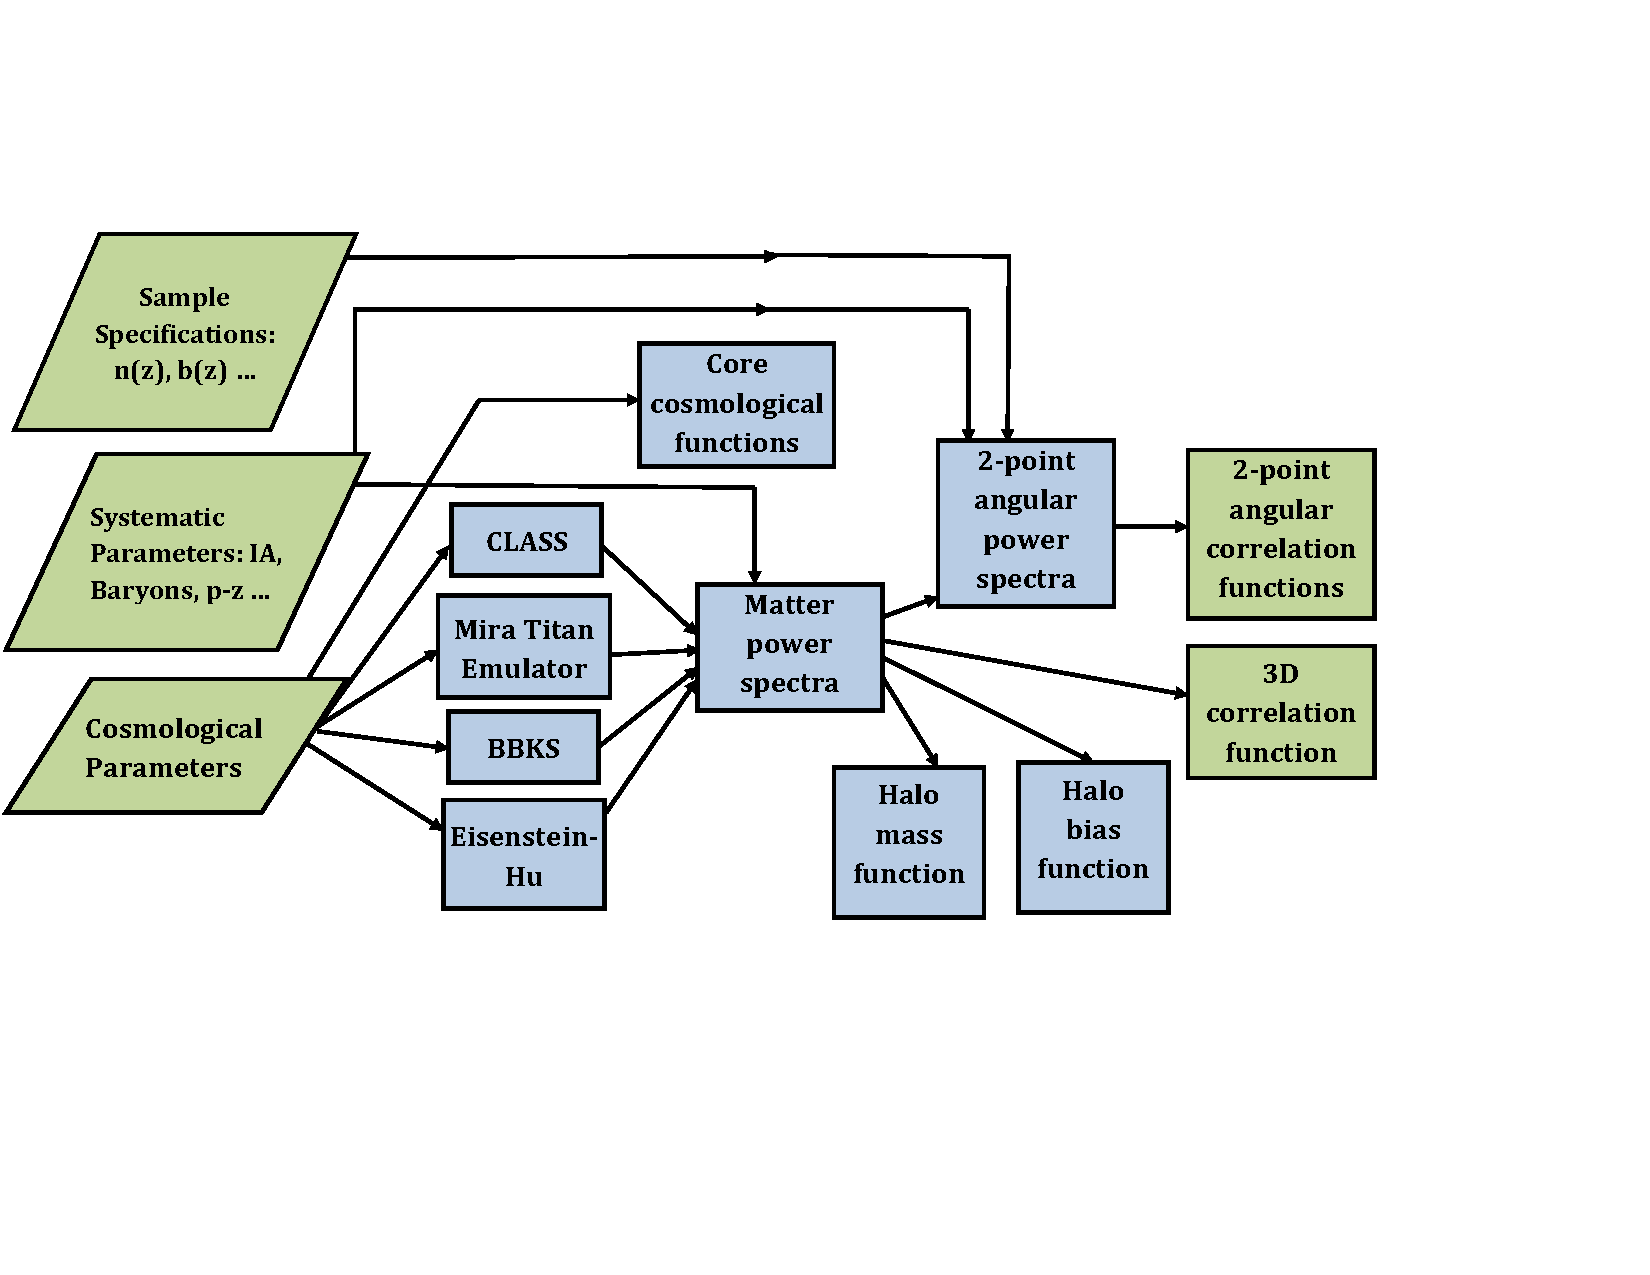
\includegraphics[width=0.9\textwidth]{CCL_Flowchart4}
\caption{\ccl structure flowchart. \ccl is written in C with a Python interface. \ccl routines calculate basic cosmological functions such as the Hubble function, density parameters, distances and growth function. It uses various methods to compute the matter-power spectrum including {\tt CLASS}, ``Cosmic Emulator'' developed by \citet{Lawrence17}, or common approximations. It computes 2-point angular power spectra and correlation functions from various probes. \ccl is designed to accommodate multiple methods to calculate cosmological observables.}
\label{fig:CCL_structure}
\end{figure*}
%------------------------

This manuscript [paper?] is organized as follows. Section \ref{sec:models} describes the cosmological models and observables supported by \ccl. In Section \ref{sec:implement}, we describe the details of the implementation of the quantities introduced in Section \ref{sec:models}. Section \ref{sec:validation} provides details of the validation tests performed and the accuracy achieved. Section \ref{sec:usage} gives brief guidelines for usage of \ccl, although we direct the reader to the software online repository, documentation and user manual for further information. We conclude in Section \ref{sec:conclusion} with an outlook towards the integration of \ccl in LSST pipelines and we outline future additions to the software. 


%-------------------------------------------------------------------------------
\section{Cosmological models and observables}
\label{sec:models}
\vol{Renee}
\revise

The overarching goal of \ccl is to allow seamless integration of different cosmological models of interest to LSST.

The cosmological components include the matter density parameter $\Omega_m$, the dark energy density $\Omega_\Lambda$, the radiation density $\Omega_g$ , the curvature density $\Omega_K$, the neutrino density of both massless and massive neutrinos, given by $\Omega_{\nu, {\rm rel}}$ and $\Omega_{\nu, {\rm m}}$ respectively, and parameters for the equation of state of dark energy defined below. The normalization of the density fluctuations is established either in terms of the amplitude of the primordial power spectrum, $A_s$, which is a power-law of index $n_s$, or in terms of the RMS variance in spheres of $8\,h/$Mpc today, $\sigma_8$. 

Currently, the following families of models are supported:
\begin{itemize}
 \item Flat $\Lambda$CDM cosmology with parameters $\Omega_b$, $n_s$, $A_s$ or $\sigma_8$, $\Omega_m$, $\Omega_\Lambda$, and a cosmological constant dark energy model with equation-of-state $w=-1$. \tom{Drop $\Omega_\Lambda$, since for flat LCDM it is always fixed by knowing $\Omega_m$.}
\item $w$CDM and the Chevallier-Polarski-Linder (CPL) model for dark energy and its redshift dependence, which adopts the following parametrization for $w$ as a function of the scale factor, $a$ (\citealt{Chevallier01} and \citealt{Linder03}),
  \begin{equation}
    w(a) = w_0+w_a(1-a).
  \end{equation}
 \item A universe with non-zero curvature ($K$) so that the curvature energy density parameter is the difference of the sum of the energy densities of the other components with respect to unity (flatness), i.e. $\Omega_K = 1- \sum_i \Omega_i$.
 \item All of the above, plus an arbitrary, user-defined modified growth function (see description in Section \ref{sec:growth}).
 \item Relativistic neutrinos in combination with any of the above, specified by $N_{\rm eff}$ (the number of relativistic neutrino species in the early Universe) and by the number of massive neutrinos today (see next item).
  \item Massive neutrino species in combination with any of the above except the user-defined modified growth function, specified by either $\Sigma m_\nu$ (which maps on to the density $\Omega_{\nu, {\rm m}}$ above), or by the individual masses of each of three neutrino species.
\end{itemize}

In the particular case of cosmologies with massive neutrinos, \ccl allows the user to specify either a sum of masses, $\Sigma m_\nu$, or the individual mass of each of three neutrino species. In the former case, \ccl will by default split $\Sigma m_\nu$ into three neutrino masses which are consistent with the normal hierarchy (see, e.g. \cite{Gerbino2017} for a review). However, the user can alternatively ask for $\Sigma m_\nu$ to be split either into masses consistent with the inverted hierarchy, or into equal masses. Each neutrino species is then checked for whether it is non-relativistic (massive) at $z=0$, and this information is used in combination with the user-provided value of $N_{\rm eff}$ (the effective number of relativistic neutrino species in the early universe) to set the number of relativistic neutrino species.

%\todo{Range of validity of the predictions.}
Not all features of \ccl are available for all models. For a guide to which predictions are available for each model, see Table \ref{tab:cosmo}. Note that if users install their own version of {\tt CLASS}, {\tt CCL} can then make predictions for a more extended set of cosmologies. Users should take care to understand the validity of the {\tt CCL} assumptions for their own models.

\begin{table*}
  \begin{center}
    \caption{Cosmologies implemented in CCL. \label{tab:cosmo}}
    \begin{tabular}{lccccccc}
      \hline\hline
      Observable/Model & flat $\Lambda$CDM & $\Lambda$CDM+$K$ & $\Lambda$CDM + $m_\nu$ & $w$CDM & $w_0+w_a$    & MG \\[3pt] 
      \hline
      Distances & \checkmark & \checkmark  & \checkmark & \checkmark & \checkmark & $X$ \\
      Growth  & \checkmark & \checkmark & $X$ & \checkmark & \checkmark & \checkmark  \\
      $P_m(k,z)$ & \checkmark & \checkmark & \checkmark & \checkmark & \checkmark & $X$\\
      Halo Mass Function & \checkmark & \checkmark & $X$ & \checkmark & \checkmark & $X$\\
      $C_l$, number counts & \checkmark & $X$ & $X$ & \checkmark & \checkmark & $X$ \\
      $C_l$, weak lensing only & \checkmark & $X$ & \checkmark & \checkmark & \checkmark & $X$ \\
      Correlation function & \checkmark & $X$ & \checkmark & \checkmark & \checkmark & $X$ \\
      \hline\hline
    \end{tabular}
  \end{center}
  %\caption{Cosmologies supported.}
\end{table*}


%\todo{Add discussion of external versions of CLASS and Modified Gravity.}

%-------------------------------------------------------------------------------
\subsection{Background cosmology}
\vol{Renee, Shahab}

The models that are specified above map directly onto cosmological observables such as the expansion rate of the Universe, which is parameterized through the Hubble parameter as
\begin{align}\label{eq:Ha}
\frac{H(a)}{H_0} &= a^{-3/2}\Big(\Omega_{m}+\Omega_{\Lambda} a^{-3(w_0+w_a)}
    \exp[3 w_a (a-1)]~+ \nonumber \\ &\Omega_{K} a + (\Omega_{g} + \Omega_{\nu, {\rm rel}}) a^{-1} + \tilde\Omega_{\nu, {\rm m}}(a)a^3\Big)^{\frac{1}{2}} ,
\end{align}
which is a function of the energy density in the different components today and the scale factor. In this expression, we have assumed the CPL parameterization described above for the dark energy equation of state, and $\tilde\Omega_{\nu, {\rm m}}(a) = \rho^{-1}_{\rm crit,0} \rho_{\nu, {\rm m}}(a)$ is the fractional energy density of massive neutrinos, calculated via
\begin{align}
\tilde\Omega_{\nu, {\rm m}}(a) &= \frac{7}{8}\sum_{i=1}^{N_\nu} \frac{4 \sigma_{B}}{c \rho_{{\rm crit},0}} \left(\frac{T_{\nu}^{\rm eff}}{a}\right)^4  \int_0^{\infty} dx \, x^2 \frac{\sqrt{x^2 + \left(\mu^i\right)^2}}{\exp(x) + 1}.
\label{Omnu}
\end{align}
Here, $\sigma_B$ is the Stefan-Boltzmann constant, $c$ is the speed of massless particles, $\rho_{{\rm crit},0}$ is the critical density at $z=0$, and $T_{\nu}^{\rm eff}$ is the present effective temperature of the massive neutrinos. $T_{\nu}^{\rm eff}$ is related to the temperature of the CMB via $T_{\nu}^{\rm eff} = T_{\rm CMB} T_{\rm NCDM}$, where $T_{\rm NCDM}$ is a dimensionless factor ($\simeq1$) used by e.g. {\tt CLASS} to set the ratio ${\sum m_\nu}/{\Omega_{\nu, {\rm m}}}$ to its experimentally measured value. Note that $T_{\rm NCDM}$ is used to modulate the effective temperature of massive neutrinos only; the temperature of relativistic neutrinos follows the usual relation. Finally, $\mu^i$ is a per-species mass-dependent dimensionless constant, given by $\mu^i = m_{\nu}^{i}c^2 a / (k_B T_{\nu}^{\rm eff})$ where $k_B$ is the Boltzmann constant.

The density parameters $\Omega_X(a)$ of a given species $X$ at a given time are defined in terms of the physical background densities $\bar\rho_X(a)$ via $\Omega_X(a) \equiv \rho^{-1}_{\rm crit}(a) \bar\rho_X(a)$, where the critical density $\rho_{\rm crit}(a) = {( 8 \pi G)}^{-1} 3c^2H^2(a) = \rho_{\rm crit,0} H_0^{-2} H^2(a)$. As an example, the physical density of matter is given by $\bar\rho_m(a) = \bar\rho_{m,0} a^{-3} = \rho_{\rm crit,0} \Omega_{m,0} a^{-3}$, and its density parameter is $\Omega_m(a) = \Omega_{m,0} H_0^{2} a^{-3} H^{-2}(a)$. \ccl moreover allows for comoving physical densities $\bar\rho_{X, {\rm com}}(a) = \bar\rho_X(a) a^3$ to be extracted, which in the case of matter reduces to $\bar\rho_{m, {\rm com}} = \rho_{\rm crit,0} \Omega_{m,0}$. We include bars for $\rho_X$ to distinguish from spatially-varying densities in later sections.

Fitting models to cosmological observables requires predicting cosmological distances for a given model. We consider the comoving radial distance, which is calculated via a numerical integral as
\begin{equation}
 \chi(a)= c \int_a^1 \frac{da'}{a'^2 H(a')}.
 \label{eq:comrdist}
\end{equation}
The comoving angular diameter distance is then computed in terms of the comoving radial distance,
\begin{equation}\label{eq:angdist}
 r(\chi)=\left\{\begin{array}{cc}
                 k^{-1/2}\sin(k^{1/2}\chi) & k>0\\
                 \chi & k=0\\
                 |k|^{-1/2}\sinh(|k|^{1/2}\chi) & k<0\\
                \end{array}\right.
\end{equation}
where $k = \left({\sum_X \Omega_X -1}\right) c^{-2} H_0^2$ is the curvature.
This function can be written directly in terms of the present curvature density parameter, $\Omega_{K,0}$, as
\begin{equation}\label{eq:angdist_omegak}
 r(\chi) = \sqrt{\Omega_{K,0}}\sinh(\sqrt{\Omega_{K,0}}\chi),
\end{equation}
which is valid for all forms of the curvature density.
The angular diameter distance is given by $d_A=a\,r(a)$, and the luminosity distance is
$d_L=r(a)/a,$ leading to the familiar relation $d_A = a^2d_L$ which is valid in general for all metric theories of gravity.
The \ccl suite also has the functionality to compute the distance modulus, defined as
\begin{equation}\label{eq:distmod}
    \mu = 5 \log_{10}(d_L / {\rm pc})-5,
\end{equation}
along with $a(\chi)$, the inverse function of $\chi(a)$.


%-------------------------------------------------------------------------------
\subsection{Growth of perturbations}
\vol{Mustapha Ishak}
\label{sec:growth}
{\textcolor{red!55!blue}{\bf Once the 2 questions below are addressed this Sub-section is ready for review.}}


Probing the growth history of the Universe can allow us to distinguish between cosmological models. 
To compute the linear growth factor of matter perturbations, $D(a)$, \ccl solves the following differential equation:
\begin{equation}
  \frac{d}{da}\left(a^3H(a)\frac{dD}{da}\right)=\frac{3}{2}\Omega_M(a)aH(a)D,
  \label{eq:growth}
\end{equation}
using a Runge-Kutta Cash-Karp algorithm. 

In doing this, \ccl simultaneously computes the logarithmic growth rate $f(a)$, defined as:
\begin{equation}
  f(a)\equiv \frac{d\ln D}{d\ln a}.
  \label{eq:lingrowthf}
\end{equation}

\ccl provides functions that return the growth normalized to $D(a=1)=1$ and to $D(a\ll1)\rightarrow a$. It employs an accelerated spline that is linearly spaced in the scale factor to interpolate the growth functions. 

The growth calculations cover flat and curved $\Lambda$CDM, $w$CDM, and $(w_0 + w_a)$CDM cosmologies. However, it should be noted that the above treatment is strictly valid for a Universe containing only dust-like matter components. A scale-independent growth rate is, for example, ill-defined in the presence of massive neutrinos; attempts to compute the growth rate in cosmologies with massive neutrinos will therefore fail by design. \jab{will \ccl crash?}

Finally, \ccl allows for an alternative `modified gravity' cosmological model defined by a regular background $(w_0+w_a)$CDM (\todo{with arbitrary $K$?}) as well as a user-defined $\Delta f(a)$, such that the true growth rate in this model is given by $f(a)=f_0(a)+\Delta f(a)$, where $f_0(a)$ is the growth rate in the background model. Note that this model is only consistently implemented with regards to the computation of the linear growth factor and growth rates.
All other \ccl functions (including the non-linear power spectrum) will ignore these modifications. This model, and the interpretation of the predictions given by \ccl, should therefore be used with care. A version of the growth code and transfer functions depending on modified gravity parameters is under development. 

%-------------------------------------------------------------------------------
\subsection{Matter power spectrum}
\label{sec:matterps}
\vol{Elisa Chisari}

Theoretical predictions for cosmological observables such as galaxy clustering, gravitational lensing and cluster mass functions rely on knowledge of the distribution of matter from small to large scales in the Universe. The quantity most frequently used to describe the distribution of matter at a given wavenumber and redshift is the matter power spectrum, $P(k,z)$, defined as
\begin{equation}
  \langle \tilde\delta({\bf k},z)\tilde\delta({\bf k}^\prime,z)\rangle = (2\pi)^3P(k,z)\
\delta_D^3({\bf k}-{\bf k}')
\end{equation}
where $\tilde\delta({\bf k})$ is the Fourier component of the overdensity field at a given wavenumber and $\delta_D^3$ is the Dirac delta function. $P(k,z)$ has units of volume and a dimensionless analogue is often defined as
\begin{equation}
  \Delta^2(k,z) \equiv \frac{k^3}{2\pi^2}P(k,z).
\end{equation}

\ccl implements several different methods for making predictions for the matter power spectrum. Two of those methods, the BBKS \citep{BBKS} and \citet{1998ApJ...496..605E} approximations, are only accurate to within a few percent and are implemented for validation purposes only. These approximations provide analytical expressions for the transfer function, $T(k)$, which is related to the matter power spectrum by $\Delta(k)^2 \propto T^2(k) k^{3+n_s}$, where $n_s$ is the power-law index of the primordial power spectrum. The normalization of the power spectrum is either defined at $z=0$ by setting $\sigma_8$ to its value today, or by setting the amplitude of primordial fluctuations, $A_s$.

The default \ccl implementation uses the {\tt CLASS} algorithm \citet{class} to obtain predictions for $P(k,z)$. In addition, \ccl can also generate $P(k,z)$ predictions by emulation of cosmological numerical simuations, in particular, using the ``Cosmic Emulator'' developed by \citet{Lawrence17}. 

None of the above methods account for the impact of baryonic physics on the distribution of matter, which is known to exceed the percent level at scales $k \gtrsim 1/$Mpc \citep{vanDaalen11,Illustris,Hellwing16,Springel17} and can affect the extraction of cosmological parameters \citep{Semboloni11,Semboloni13,Mohammed14,Eifler15,Mohammed17}. To account for this effect, we incorporate in \ccl an effective parametrization \citep{Schneider15} of the redistribution of matter as a consequence of feedback from Active Galactic Nuclei and adiabatic cooling. We give an overview of each method to predict the matter power spectrum in what follows.

{\bf BBKS approximation}. \ccl implements the analytical BBKS approximation to the transfer function \citep{BBKS}, given by
\begin{eqnarray}
  \label{eq:bbks}
  T&&(q\equiv k/\Gamma h {\rm Mpc}^{-1}) = \frac{\ln[1+2.34q]}{2.34q}\times\\
  &&[1+3.89q+(16.2q)^2+(5.47q)^3+(6.71q)^4]^{-0.25}\nonumber
\end{eqnarray}
where $\Gamma = \Omega_m h$. The BBKS power spectrum option is primarily used as a precisely-defined input for testing the numerical accuracy of \ccl routines (as described in Sec.~\ref{sec:implement}),
and it is not recommended for other uses.

{\bf Eisenstein \& Hu approximation}. \ccl also provides an approximation to the matter power spectrum as implemented by \citet{1998ApJ...496..605E} (we refer the reader to this paper for a detailed discussion of the fitting formulae).\footnote{Note that the implementation in \ccl modifies Eq. 5 of \citet{1998ApJ...496..605E} using $a^{-1}=1+z$ instead of the approximation $a^{-1}\sim z$. The difference in the resulting power spectra is negligible, but larger than 1 part in $10^4$ for $k<10\,h\,{\rm Mpc}^{-1}$.}

{\bf \tt CLASS.} The default configuration of \ccl adopts predictions for the linear and nonlinear matter power spectrum from the publicly available software \citep{class}. {\tt CLASS} currently computes the non-linear power spectrum using the HaloFit prescription of \cite{CLASS_halofit}.

{\bf Cosmic emulator.} \todo{In the section on the HMF and halo bias below, there is a lot of emphasis on the fact that these quantities are not themselves without significant uncertainty. Should we include a sentence or two to that effect here as well? - DL} \jab{my general comment in the abstract is related to this.} \tom{I think we should avoid all discussions of physical accuracy and near the top say ``all models presented in the paper (P, HMF, bias, etc.) are themselves physically uncertain. The reader should consult those papers to learn about the physical accuracy.''} The emulator \citep{Lawrence17} provides accurate predictions for the nonlinear matter power spectrum, at the $1\%$ level for $z\leq 2$ and in the wavenumber range $k=[10^{-3},5]$ Mpc$^{-1}$. The allowed range of cosmological parameters that can be passed to the emulator is as follows:
 \begin{eqnarray}
 0.12&\leq& \Omega_{m} h^2 \leq 0.155,\nonumber\\
 0.0215&\leq& \Omega_{b} h^2 \leq 0.0235,\nonumber\\
 0.7&\leq& \sigma_8 \leq 0.9,\nonumber\\
 0.55&\leq& h \leq 0.85,\nonumber\\
 0.85&\leq& n_s\leq 1.05,\nonumber\\
 -1.3&\leq& w_0\leq-0.7,\nonumber\\
 -1.73&\leq& w_a\leq -0.7,\footnote{$w_a$ and $w_0$ are constrained jointly to be $0.3\leq (-w_0-w_a)^{1/4}$.}\nonumber\\
 0.0&\leq& \Omega_{\nu, {\rm m}} h^2 \leq 0.01.
 \end{eqnarray}
In the case of the emulator, the effective number of relativistic neutrino species is set to $N_{\rm eff}=3.04$. In \citet{Lawrence17}, the neutrino component of the power spectrum is not simulated, but either linearly evolved and added to the simulated power spectra at low redshift, or accounted for by a scale-dependent correction to the growth function. More details on this method and its accuracy can be found in \citep{Upadhye14,Castorina15,Heitmann16}.
 
 {\bf Baryonic correction model (BCM).} \ccl incorporates the impact of baryons on the total matter power spectrum via the BCM of \citet{Schneider15}. The main consequences of baryonic processes are: to suppress the power spectrum at intermediate scales ($k\sim$ a few $h/$Mpc) due to the ejection of gas by Active Galactic Nuclei feedback, and to enhance it at smaller scales due to adiabatic cooling. To account for these effects, BCM uses an effective decomposition for the impact of gas ejection ($G$) and the enhancement of the small scale profile due to star formation ($S$) to estimate the fractional effect of baryonic processes on the dark matter-only power spectrum ($P_{\rm DMO}$):
\begin{equation}
  P_{\rm BCM}(k,z)=P_{\rm DMO}(k,z) G(k|M_c,\eta_b,z)S(k|k_s)
\end{equation}
Three effective parameters govern the contribution of baryonic processes to modifying the total matter power spectrum:
 \begin{itemize}
   \item $\log_{10} [M_c/($M$_\odot/h)]$: the mass of the clusters responsible for feedback, which regulates the amount of suppression of the matter power spectrum at intermediate scales;
   \item $\eta_b$: a dimensionless parameter which determines the scale at which suppression peaks;
   \item and $k_s$ [$h/$Mpc]: the wavenumber that determines the scale of the stellar distribution of matter in the center of halos.
 \end{itemize}
 If these parameters are not specified by the user, \ccl assumes the default parameters of \citet{Schneider15}, calibrated through different comparisons with observations and simulations in that work.

%-------------------------------------------------------------------------------
\subsection{Two-point correlators}
\vol{David Alonso, Tom McClintock}

This section describes the theoretical expectations for the two-point correlators of pairs of quantities (fields) defined on the sky. These fields can be classified in terms of their spin $s$ under rotations on the plane tangent to the sphere. In general a spin-$s$ field is defined by two real-valued functions of the spherical coordinates $a_1(\nv)$ and $a_2(\nv)$ (e.g. $\gamma_1$ and $\gamma_2$ for weak lensing or the Stokes parameters $Q$ and $U$ in the case of polarized intensity), from which one can form the complex field $a=a_1+ia_2$.

Spin-$s$ quantities can be decomposed into their harmonic coefficients $\,_sa_{\ell m}$ through a spherical harmonic transform:
\begin{equation}\nonumber
  \,_sa_{\ell m}=\int d\nv\,a(\nv)\,_sY^*_{\ell m}(\nv),\hspace{12pt}
  a(\nv)=\sum_{\ell m}\,_sa_{\ell m}\,Y_{\ell m}(\nv)
\end{equation}
where $_sY_{\ell m}$ are the spin-weighed spherical harmonics. The harmonic coefficients can then be associated with parity-even and parity-odd components ($E$-modes and $B$-modes respectively) as\footnote{We note that for spin-$0$ quantities the minus sign preceding these equations is usually omitted.}
\begin{align}\nonumber
   E_{\ell m}&=-\frac{1}{2}\left[\,_{s}a_{\ell m}+(-1)^s\,_{-s}a_{\ell m}\right]\\\nonumber
  iB_{\ell m}&=-\frac{1}{2}\left[\,_{s}a_{\ell m}-(-1)^s\,_{-s}a_{\ell m}\right]
\end{align}

In what follows we will focus on scalar ($s=0$) quantities such as the overdensity of source number counts or the lensing convergence, and on spin-2 fields such as the lensing shear. We will also distinguish between {\sl tracers} (fields observed on the sky, such as number counts in a redshift bin, shear, or CMB temperature fluctuations) and {\sl contributions} to the total observed fluctuations of these tracers (such as the biased matter density term in number counts, redshift-space distortions, magnification, etc.).

\subsubsection{Angular power spectra}\label{sssec:2pt.pspec}
\vol{David Alonso}

The angular power spectrum $C^{ab}_\ell$ between two tracers $a$ and $b$ is defined as
\begin{equation}
  \langle a_{\ell m}b^*_{\ell m}\rangle\equiv C^{ab}\delta_{\ell\ell'}\delta_{mm'},
\end{equation}
where $a_{\ell m}$ and $b_{\ell m}$ can be either the $E$-mode or $B$-mode component of the corresponding field. In what follows we will only deal with fields for which the $B$-modes are identically $0$, and therefore all equations refer to the $E$-$E$ power spectrum. In general, this power spectrum can be written as:
\begin{equation}
  C^{ab}_\ell=4\pi\int_0^\infty \frac{dk}{k}\,\mathcal{P}_\Phi(k)\Delta^a_\ell(k)\Delta^b_\ell(k),
  \label{eq:cls}
\end{equation}
where $\mathcal{P}_\Phi(k)$ is the dimensionless power spectrum of the primordial curvature perturbations, and $\Delta^a$ and $\Delta^b$ are the transfer functions corresponding to these tracers. Each transfer function will receive contributions from different terms. Currently \ccl supports three types of tracers: number counts, galaxy shape distortions and lensing convergence, with the following contributions:

\paragraph{\bf Number counts.} The transfer function for number counts can be decomposed into three contributions: $\Delta^{\rm NC}=\Delta^{\rm D}+\Delta^{\rm RSD}+\Delta^{\rm M}$, where
\begin{itemize}
  \item $\Delta^{\rm D}$ is the standard density term proportional to the matter density:
        \begin{equation}\label{eq:transfer_nc}
          \Delta^{\rm D}_\ell(k)=\int dz\,p_z(z)\,b(z)\,T_\delta(k,z)\,j_\ell(k\chi(z)),
        \end{equation}
        where $j_\ell(x)$ is $\ell$-th order spherical Bessel function, $T_\delta$ is the matter transfer function, $b(z)$ is the linear clustering bias for this tracer and $p_z(z)$ is the normalized distribution of sources in redshift (i.e. the selection function). The fluctuations in the number density of sources in different redshift bins are therefore treated by \ccl as different tracers. Note that \ccl currently does not support non-linear or scale-dependent bias, but future releases will do so under a number of schemes, including perturbative approaches as implemented in e.g. \cite{FASTPT}.
  \item $\Delta^{\rm RSD}$ is the linear contribution from redshift-space distortions (RSDs):
        \begin{equation}\label{eq:transfer_rsd}
          \Delta^{\rm RSD}_\ell(k)=\int dz\,\frac{(1+z) p_z(z)}{H(z)}T_\theta(k,z) j_\ell''(k\chi(z)),
        \end{equation}
        where $T_\theta(k,z)$ is the transfer function of $\theta$, the divergence of the comoving velocity field,and $j''_\ell$ is the second order derivative of the spherical Bessel function, $j_\ell$. Note that the RSD contribution to number counts is currently computed by \ccl assuming a linear-theory relation between the matter overdensity and peculiar velocity fields, mediated by the scale-independent growth rate $f$. While this should not be problematic for wide photometric redshift bins and standard cosmological models, users should exercise care when interpreting results for narrow window functions or exotic cosmologies. Additionally, number count tracers with RSD in cosmologies with massive neutrinos are not currently supported.
  \item $\Delta^{\rm M}$ is the contribution from lensing magnification:
        \begin{align}\nonumber
          \Delta_\ell^{\rm M}(k)=-\ell(\ell+1)\int & \frac{dz}{H(z)} W^{\rm M}(z) \\\label{eq:deltaM}
          &T_{\phi+\psi}(k,z) j_\ell(k\chi(z)),
        \end{align}
        where $T_{\phi+\psi}$ is the transfer function for the Newtonian-gauge scalar metric perturbations, and $W^{\rm M}$ is the magnification window function:
        \begin{equation}
          W^{\rm M}(z)\equiv\int_z^\infty dz'\,p_z(z')\frac{2-5s(z')}{2}\frac{r(\chi'-\chi)}{r(\chi')r(\chi)}.
        \end{equation}
        Here, $s(z)$ is the magnification bias, given as the logarithmic derivative of the number of sources with magnitude limit, and $r(\chi)$ is the angular comoving distance (see Eq. \ref{eq:angdist}).
\end{itemize}
Note that \ccl currently does not compute relativistic corrections to number counts \citep{2011PhRvD..84d3516C,2011PhRvD..84f3505B}. Although these will be included in the future, their contribution to the total fluctuation is largely subdominant (see \cite{GReffects} and the two references above), and therefore it is safe to ignore them for our purposes.

\paragraph{\bf Correlated galaxy shapes.} The transfer function for correlated galaxy shapes (intrinsic and lensed) is currently decomposed into two terms: $\Delta^{\rm SH}=\Delta^{\rm WL}+\Delta^{\rm IA}$, where
\begin{itemize}
  \item $\Delta^{\rm L}$ is the standard lensing (``cosmic shear'') contribution:
    \begin{align} \label{eq:transfer_lensing}
      \nonumber
      \Delta_\ell^{\rm L}(k)=-\frac{1}{2}\sqrt{\frac{(\ell+2)!}{(\ell-2)!}}\int &\frac{dz}{H(z)} W^{\rm L}(z)T_{\phi+\psi}(k,z)\\
      &j_\ell(k\chi(z)),
    \end{align}
    where $W^{\rm L}$ is the lensing kernel, given by
    \begin{equation}
      W^L(z)\equiv\int_z^\infty dz' p_z(z')\frac{r(\chi'-\chi)}{r(\chi')r(\chi)}.
    \end{equation}
  \item $\Delta^{\rm IA}$ is the transfer function for intrinsic galaxy alignments. \ccl currently supports the so-called ``non-linear alignment model'', in which the intrinsic galaxy inertia tensor is proportional the local tidal tensor \cite{2004PhRvD..70f3526H,2007MNRAS.381.1197H}:
    \begin{align}\nonumber
      \Delta_\ell^{\rm IA}(k)=\sqrt{\frac{(\ell+2)!}{(\ell-2)!}}\int &dz\,p_z(z)\,b_{\rm IA}(z)\,f_{\rm IA}(z)\\
      &T_\delta(k,z)\,\frac{j_\ell(k\chi(z))}{[k\chi(z)]^2}.
    \end{align}
    Here, $b_{\rm IA}$ is the so-called alignment bias, and $f_{\rm IA}$ is the fraction of aligned galaxies in the sample. Notice that $b_{\rm IA}(z)$ absorbs the typical normalization factors used in the literature for intrinsic alignment amplitude and redshift evolution. It is thus not to be confused with $C_1$ or $A_{\rm IA}$, typical parameters for the linear alignment model, as adopted in works such as \cite{Blazek17,vanUitert18,Joudaki18,Hildebrandt17}.
\end{itemize}

\paragraph{\bf Lensing convergence.} The transfer function for the lensing convergence of a given source plane at redshift $z_*$ receives only one contribution, given by
\begin{equation}
  \Delta_\ell^\kappa(k)=-\frac{\ell(\ell+1)}{2}\int_0^{\chi_*}\frac{dz}{H(z)}\,\frac{r(\chi_*-\chi)}{r(\chi)r(\chi_*)}T_{\phi+\psi}(k,z),
  \label{eq:cmblens}
\end{equation}
where $\chi_*\equiv\chi(z_*)$.

\noindent
It is worth noting that the equations above should be modified for non-flat cosmologies by replacing the spherical Bessel functions $j_\ell$ with their hyperspherical counterparts \citep{1994ApJ...432....7K}. These are currently not supported by \ccl \todo{Clarify in Table 1?}, and their impact is mostly relevant on low multipoles. The library also assumes a factorizable matter power spectrum at unequal times $P_\delta(k,z_1,z_2)=T_\delta(k,z_1)T_\delta(k,z_2)\,2\pi^2\mathcal{P}_\Phi(k)$ (see \citealt{2017PhRvD..95f3522K}). Furthermore, \ccl currently assumes a relation between transfer functions $T_\delta$, $T_\theta$ and $T_{\phi+\psi}$ that is strictly only valid in vanilla $\Lambda$CDM:
\begin{equation}
  T_\delta=-\frac{1+z}{H(z)f(z)}T_\theta=-\frac{k^2}{3H_0^2\Omega_M}\frac{T_{\phi+\psi}}{1+z}.
\end{equation}
These approximations will be revisited in future versions of the library. \jab{It appears we are defining the transfer function to include both the early universe physics and late-time nonlinear growth. Perhaps we should clarify this to avoid confusion with the standard linear theory transfer function.}


\subsubsection{Correlation functions}
\vol{Elisa Chisari, Sukhdeep Singh}


Fields can also be correlated in configuration space, and the corresponding correlators are called correlation functions. Let $a$ and $b$ be two fields with spins $s_a$ and $s_b$. We start by defining $\tilde{a}(\nv_1)$ and $\tilde{b}(\nv_2)$ as the fields $a$ and $b$ rotated such that the $x$-axis of the tangential coordinate systems at $\nv_1$ and $\nv_2$ become aligned with the vector connecting both points. We can then define two correlation functions:
\begin{equation}\nonumber
  \xi^{ab}_+(\theta)\equiv\left\langle\tilde{a}(\nv_1)\tilde{b}^*(\nv_2)\right\rangle,\hspace{12pt}
  \xi^{ab}_-(\theta)\equiv\left\langle\tilde{a}(\nv_1)\tilde{b}(\nv_2)\right\rangle,
  \label{eq:xipm}
\end{equation}
where $\nv_1\cdot\nv_2\equiv\cos\theta$. 

$\xi_{\pm}$ can be related to the power spectra as
\begin{equation}\label{eq:cl_xi}
 \xi^{ab}_\pm = \sum_\ell\frac{2\ell+1}{4\pi}\,(\pm1)^{s_b}\,C^{ab\pm}_\ell\,d^\ell_{s_a,\pm s_b}(\theta),
\end{equation}
where $d^\ell_{mm'}$ are the Wigner-$d$ matrices \citep{Ng1999,2004MNRAS.350..914C} and we have defined the power spectra
\begin{equation}
  C^{ab\pm}_\ell\equiv\left(C^{a_Eb_E}_\ell\pm C^{a_Bb_B}_\ell\right)+i\left(C^{a_Bb_E}_\ell\pm C^{a_Eb_B}_\ell\right),
\end{equation}
which reduces to the $EE$ power spectrum when all $B$-modes are 0.

Note that, as scalar quantities are real, any correlation involving at least one spin-$0$ field only has one non-unique correlation function. In these cases, the Wigner-$d$ matrices can also be expressed in terms of associated Legendre polynomials $P^m_\ell$, and therefore Eq. \ref{eq:cl_xi} becomes
\begin{align}
  \xi^{ab}(\theta)&=\sum_\ell\frac{2\ell+1}{4\pi}\,C^{ab}_\ell\sqrt{\frac{(\ell-s_a)!}{(\ell+s_a)!}}P^{s_a}_\ell(\cos\theta)\\
                  &=\sum_\ell\frac{2\ell+1}{4\pi}\,C^{ab}_\ell P_\ell(\cos\theta),
\label{eq:xigg}
\end{align}
where the last equality holds for $s_a=0$, and both expressions assume $s_b=0$.

In the flat-sky approximation we can take the small-scale limit $\ell\gg s_1,s_2$ and approximate 
\begin{equation}
  d_{s_1s_2}^\ell(\theta)\longrightarrow J_{s_1-s_2}(\ell\theta),
\end{equation}
where $J_\alpha(x)$ is the Bessel function of order $\alpha$. Eq. \ref{eq:cl_xi} then becomes\footnote{See the weak lensing review by \citet{Bartelmann01}, page 44 and \citet{Joachimi10}.}
\begin{equation}
  \xi^{ab}_{\pm}(\theta)=\left(\pm1\right)^{s_b}\int\frac{d\ell\,\ell}{2\pi}\,C^{ab\pm}_\ell J_{s_a\mp s_b}(\ell\theta).
\end{equation}

In summary, for spins 0 and 2, the three relevant cases for the cosmological observables supported by \ccl are:
\begin{itemize}
  \item $s_a=s_b=0$ (e.g. galaxy-galaxy, galaxy-$\kappa$ and $\kappa$-$\kappa$):
    \begin{align}\label{eq:xi00full}
      \xi^{ab}(\theta)&=\sum_\ell\frac{2\ell+1}{4\pi}\,C^{ab}_\ell P_\ell(\cos\theta)\hspace{5pt}\text{(full-sky)}\\\label{eq:xi00flat}
                      &=\int_0^\infty\frac{d\ell\,\ell}{2\pi}\,C^{ab}_\ell J_0(\ell\theta)\hspace{25pt}\text{(flat-sky)}
    \end{align}
  \item $s_a=2$, $s_b=0$ (e.g. galaxy-shear, $\kappa$-shear):
    \begin{align}\label{eq:xi02full}
      \xi^{ab}(\theta)&=\sum_\ell\frac{2\ell+1}{4\pi}\,C^{ab}_\ell d^\ell_{2,0}(\theta)\hspace{15pt}\text{(full-sky)}\\\label{eq:xi02flat}
                      &=\int_0^\infty\frac{d\ell\,\ell}{2\pi}\,C^{ab}_\ell J_2(\ell\theta)\hspace{25pt}\text{(flat-sky)}
    \end{align}
  \item $s_a=s_b=2$ (e.g. shear-shear):
    \begin{align}\label{eq:xi22full}
      \xi^{ab}_\pm(\theta)&=\sum_\ell\frac{2\ell+1}{4\pi}\,C^{ab}_\ell d^\ell_{2,\pm2}(\theta)\hspace{12pt}\text{(full-sky)}\\\label{eq:xi22flat}
                      &=\int_0^\infty\frac{d\ell\,\ell}{2\pi}\,C^{ab}_\ell J_{2\mp2}(\ell\theta)\hspace{16pt}\text{(flat-sky)}
    \end{align}
\end{itemize}

\subsubsection{3-dimensional spatial correlation function.}
In addition to the angular correlation functions, \ccl can also be used to compute the three-dimensional spatial correlation function, $\xi(r)$, from the transform of the matter power spectrum:
\begin{equation}
\xi(r) = \frac{1}{2 \pi^2} \int dk \; k^2 P(k) \frac{\sin(kr)}{kr}
\label{eq:xi3d}
\end{equation}
In the future \ccl will be expanded to incorporate the calculation of the higher-order multipoles needed to characterize the redshift-space three-dimensional correlation function in the presence of RSDs.


%-------------------------------------------------------------------------------
\subsection{Halo mass function}
\vol{Antonio Villarreal, Tom McClintock}

Being able to calculate the halo abundance as a function of mass is a necessary step to being able to constrain cosmology with probes such as galaxy clusters. While analytic functions are the traditional means of predicting evolution of halo abundances, calibration is frequently required against cosmological simulations. In order to reach the high precision required for cosmological constraints in a self-consistent fashion, it is ultimately necessary to use cosmological simulations; we implement this with halo mass functions with parameters fit to these simulations. The calculation of the halo mass function focuses around the spherical overdensity method of halo finding, in which the size of a halo can be defined with:

\begin{equation}
\bar{\rho}(r_{\Delta}) = \Delta \times \bar{\rho}_{\mathrm{m}},
\end{equation}
%
where a spherical halo with radius $r_{\Delta}$ has an average density $\bar{\rho}$ equal to the overdensity parameter $\Delta$ times the mean background density of the universe at a given redshift, $\bar\rho_{\mathrm{m}}(z)$. Within the literature, the choice of $\Delta$ can vary considerably, as observations focusing on the compact cores of halos often take much larger values of $\Delta$ than the fiducial definition in most halo clustering studies, $\Delta = 200$. We note that another common definition exists which utilizes the critical density of the universe, $\rho_{\mathrm{crit}}$; this introduces a simple conversion factor between the two definitions that must be accounted for. Currently, \ccl only accepts overdensity parameters with respect to the mean matter density, but we plan to allow for self-consistent handling of critical density based definitions in the future.

The halo mass function is defined as
\begin{equation}
\frac{dn}{dM}=f(\sigma)\frac{\bar{\rho}_\mathrm{m}}{M}\frac{d\ln{\sigma^{-1}}}{dM},
\label{eq:halo_mass_function}
\end{equation}
where $n$ is the number density of halos of a given mass $M$ associated with the RMS variance of the matter density field $\sigma^2$ at a given redshift and $f$ is the derived fitting function\footnote{Not to be confused with the linear growth rate of structure defined in Eq. \ref{eq:lingrowthf}}. In \ccl calling this function returns the mass function in logarithmic mass bins, $dn/d\log_{10}{M}$, where the input is the halo mass $M$ and scale factor $a$.

The halo mass $M$ is related to $\sigma$ by first computing the radius $R$ that would enclose a mass $M$ in a homogeneous Universe at $z=0$:
\begin{equation}
  M=\frac{H_0^2}{2G}R^3\,\rightarrow \frac{M}{M_\odot}=1.162\times10^{12}\Omega_Mh^2\,\left(\frac{R}{1\,{\rm Mpc}}\right)^3.
\end{equation}
The RMS density contrast in spheres of radius $R$ can then be computed as
\begin{equation}
  \sigma_R^2 = \frac{1}{2\pi^2}\int dk\,k^2\,P(k)\,\tilde{W}_R^2(k)
  \label{eq:sigR}
\end{equation}
where $P(k)$ is the linear matter power spectrum and $\tilde{W}(kR)$ is the Fourier transform of a spherical top hat window function,
\begin{equation}
\tilde{W}_R(k) = \frac{3}{(kR)^3}[\sin(kR)-kR\cos(kR)].
\end{equation}

This is commonly related in terms of the mass inside of the Lagrangian scale of the halo, using the following transformation:
\begin{equation}
R = (3M/4\pi{\bar\rho_{\mathrm{m}}})^{1/3}.
\end{equation}
As a consequence, one can also define $\sigma_M$ as the RMS variance of the density field smoothed on some scale $M$, analogously to Eq.(\ref{eq:sigR}).

One commonly used halo mass function definition within the literature is the \citet{Tinker2010} fitting function. This fitting function has been developed using collisionless $N$-body simulation data, using halos identified by spherical overdensities. This is an extension of the \citet{Tinker2008} halo mass function, which is also included within \ccl as a comparative option. This fitting function assumes little change with respect to cosmological parameters. Further, it includes a redshift scaling which is assumed to sharply end at a redshift of $z = 3$. This halo mass function is calibrated within the range of $10^{10.5} h\mathrm{M}_\odot \leq M \leq 10^{15.5} h\mathrm{M}_\odot$ at a redshift of $z = 0$.

For comparison purposes, we also have included the results of \citet{Angulo2012}, which uses the Millenium XXL simulation in order to study galaxy cluster scaling relations. As part of this study, they have calculated their own fit to the \citet{Tinker2010} fitting function. While this additional halo mass function is available, it has not been extended to a broad range of overdensity parameter $\Delta$, nor has it been extended beyond a redshift of $z = 0$.

The \citet{Tinker2008} fitting function uses the following parameterisation:
\begin{equation}
f(\sigma)=A\Big[\Big(\frac{\sigma}{b}\Big)^{-a}+1\Big]e^{-c/{\sigma}^2},
\end{equation}
where $A$, $a$, $b$, and $c$ are fitting parameters that have additional redshift scaling. This basic form is modified for the \citet{Angulo2012} formulation. The resulting form is
\begin{equation}
f(\sigma)=A\Big[\Big(\frac{b}{\sigma}+1\Big)^{-a}\Big]e^{-c/{\sigma_M}^2},
\end{equation}
where the only change is in the formulation of the second term. Note that the fitting parameters in the \citet{Angulo2012} formulation do not contain any redshift dependence and the use of it is primarily for testing and benchmark purposes.

The \citet{Tinker2010} model parameterizes the halo mass function in terms of the peak height, $\nu = \delta_c/\sigma_M$, where $\delta_c=1.686$ is the critical density for collapse. The function is then re-expressed as
\begin{equation}
  f(\nu) = \alpha[1+(\beta\nu)^{-2\phi}]\nu^{2\eta}e(-\gamma\nu^2/2).
\end{equation}

We note that these halo mass functions, while implemented to high {\em numerical} accuracy through comparison against a flat $\Lambda$CDM cosmology (see `CCL1' in Table  \ref{tab:cosmologies}), carry their own uncertainties. It has not been significantly studied whether the halo mass function is universal with respect to changes in dark energy parameterisation.
%Further, \citet{Tinker2010} found a $\sim6\%$ scatter when determining the halo bias due to differences in simulations.
%This is in addition to a $5\%$ error in the mass function alone.
\citet{Tinker2008,Tinker2010} quote 5\% accuracy of their mass funcitons.
This result is consistent with the work of \citet{Watson2013}, which also finds a $5\%$ level difference in comparison to the Tinker fitting function. Further study will be required in the future in order to gain percent level accuracy in determining the halo mass function.\todo{For what cosmologies was the Tinker mass function tested? I.e., what should go in Table 1?}

\subsection{Halo bias}
\vol{Antonio Villarreal}

\jab{I'm a bit confused by this section. This is a quantity that CCL can return. But currently the clustering observables can only handle linear (scale-independent) bias? And should we say that the user can specify a linear bias that does not come from this fitting formula?}
\asv{Including the Tinker fitting function for the halo bias is a fairly natural step considering we are also including the Tinker mass function (on which this is heavily related to). I do not think the fact that the clustering section of the code is currently unready to handle more than linear bias impacts the usefulness of having this built in. That being said, I will specify that currently we do not have a linear bias model built in as an explicit framework, though it can certainly be passed in to other sections of the code.}

An important step in many interpretations of the halo model is to have a measure of the bias of dark matter halos, defined as the ratio of the halo power spectrum to the linear dark matter power spectrum,
\begin{equation}
  b^2(k) = \frac{P_h(k)}{P_{\mathrm{lin}}(k)}.
  \label{eq:halo_bias}
\end{equation}

As with measures of the halo mass function, high accuracy cosmological constraints requires the use of numerical simulations to develop fitting functions and emulators. We note that we will define haloes as in the above subsection focusing on the halo mass function. {\tt CCL} currently implements the halo bias fitting function results in \citet{Tinker2010}, though future improvements will likely require the use of emulator methods.

The \citet{Tinker2010} model parameterizes the halo mass function and the halo bias in terms of the peak height and the critical density for collapse as
\begin{eqnarray}
  b(\nu) &=& 1 - A\frac{\nu^a}{\nu^a + {\delta_c}^a} + B\nu^b+C\nu^c,\\
  f(\nu) &=& \alpha[1+(\beta\nu)^{-2\phi}]\nu^{2\eta}e(-\gamma\nu^2/2).
\end{eqnarray}

Again, while high {\em numerical} accuracy has been verified, there is a remaining uncertainty. \citet{Tinker2010} found a $\sim6\%$ scatter when determining the halo bias due to differences in simulations alone. In addition, this parameterization does not include a careful exploration of any impact due to changes in the dark energy equation of state. As with the halo mass function, studies will be required to reach accuracy at the percent level for any cosmological predictions. 

We note that many observables are currently tuned to utilizing a linear halo bias (e.g. scale independent). While the current functionality of {\tt CCL} is to return the \citet{Tinker2010} model for halo bias, it is entirely possible to generate simpler models of halo bias and pass this into further functions.

\subsection{Halo model}
\label{sec:halo_model}
\vol{Alexander Mead}
\todo{This section will most likely be commented out.}

In this section we review a basic halo-model computation \citep{Seljak2000,Peacock2000,Cooray2002} of the cross-correlation between any two cosmological fields and only requires knowledge of the halo profiles of the field in question. For example, in the case of the matter-density auto spectrum we need only know the halo density profiles. For the galaxy spectrum we require knowledge of the number of, and distribution of, galaxies as a function of halo mass. In this simple form the halo model is approximate and makes the assumption that haloes are \emph{linearly} biased with respect to the \emph{linear} matter field and also assumes that haloes are spherical with properties that are determined solely by the halo mass. It is possible to go beyond these simplified assumptions, and we direct the interested reader to \cite{Cooray2002,Smith2007,Giocoli2010,Smith2011}.

The eventual aim for CCL is to have a halo model that can calculate the auto- and cross-spectra for any cosmological field combinations with parameters that can be taken either from numerical simulations or observational data. Currently we have only implemented the case of the matter-density auto spectrum, but we keep the notation as general as possible in the following:

Consider two 3D cosmological fields $\rho_i$ and $\rho_j$, the cross power spectrum at a given redshift can be written as a sum of a two- and a one-halo term given by
\begin{equation}
P_{2\mathrm{H},ij}(k)=P_{\mathrm{lin}}(k)
\prod_{n=i,j}\left[\int_0^\infty b(M)\frac{\mathrm{d}n}{\mathrm{d}M}W_n(M,k)\;\mathrm{d}M\right]\ ,
\label{eq:two_halo}
\end{equation}
\begin{equation}
P_{1\mathrm{H},ij}(k)=\int_0^\infty \frac{\mathrm{d}n}{\mathrm{d}M}W_i(M,k)W_j(M,k)\;\mathrm{d}M\ ,
\label{eq:one_halo}
\end{equation}
where $M$ is the halo mass, $\mathrm{d}n/\mathrm{d}M$ is the halo mass function defined in equation~(\ref{eq:halo_mass_function}) and $b(M)$ is the linear halo bias with respect to the linear matter density field, defined as the large-scale limit of equation~(\ref{eq:halo_bias}).

Equations~(\ref{eq:two_halo}) and (\ref{eq:one_halo}) contain the (spherical) Fourier transform of the halo profile, or halo `window function':
\begin{equation}
W_i(M,k)=\int_0^\infty4\pi r^2\frac{\sin(kr)}{kr}\rho_{\mathrm{H},i}(M,r)\;\mathrm{d}r\ ,
\label{eq:window_function}
\end{equation}
where $\rho_{\mathrm{H},i}(M,r)$ is the radial profile for the field $i$ in a host halo of mass $M$. For example, if one is interested in matter fields then this would be the halo density profile, if one were interested in galaxies then this would be the number density and distribution of galaxies around a halo of mass $M$.

%The dimensionless mass function, $f(\nu)$, is related to $n(M)$ via
%\begin{equation}
%f(\nu)\,\mathrm{d}\nu=\frac{M}{\bar\rho}n(M)\;\mathrm{d}M\ .
%\label{eq:mass_function}
%\end{equation}
%and is written in terms of the mass variable $\nu=\delta_\mathrm{c}/\sigma(M)$: $\delta_\mathrm{c}$ is the critical linear density for halo collapse: $\delta_\mathrm{c}\simeq 1.686$, but with a weak cosmology dependence.  $\sigma(M)$ is the variance in the linear matter field when filtered on a Lagrangian scale $R$ corresponding to mass $M=4\pi R^3/3$:
%\begin{equation}
%\sigma^2(R)=\int_0^{\infty}\Delta_{\mathrm{lin}}^2(k)\, T^2(kR)\;\mathrm{d}\ln{k}\ ,
%\label{eq:variance}
%\end{equation}
%with $T$ being the Fourier Transform of a real-space top-hat filter
%\begin{equation}
%T(x)=\frac{3}{x^3}(\sin{x}-x\cos{x})\ .
%\label{eq:top_hat}
%\end{equation}
Note that the halo mass function and bias \emph{must} satisfy the following properties for the total power spectrum to have the correct large-scale limit\footnote{Note that achieving these correct limits for some fields is difficult numerically because of the large amount of mass contained in low mass haloes according to most popular mass functions. Special care must be taken with the two-halo integral in the case of matter power spectra.}:
\begin{equation}
\frac{1}{\bar\rho_\mathrm{m}}\int_0^\infty M\frac{\mathrm{d}n}{\mathrm{d}M}\;\mathrm{d}M=1\ ,
\label{eq:mf_normalisation}
\end{equation}
\begin{equation}
\frac{1}{\bar\rho_\mathrm{m}}\int_0^\infty Mb(M)\frac{\mathrm{d}n}{\mathrm{d}M}\;\mathrm{d}M=1\ .
\label{eq:bias_normalisation}
\end{equation}
If one uses a mass function and bias pair that are related via the peak-background split formalism \citep{Mo1996,Sheth2001} the these conditions are automatically satisfied. In words these equations enforce that all matter is associated to a halo and that matter is on average unbiased with respect to itself. In the convention used in CCL the units of $P(k)$ will be exactly the units of $\rho_i\rho_j / \mathrm{Mpc}^3$. The units of the $W_i$ are those of $\rho_i$ multiplied by volume.

For the matter power spectrum we use the halo profiles of \citeauthor*{Navarro1997} (NFW; \citeyear{Navarro1997}):
\begin{equation}
\rho_\mathrm{H}(M,r)\propto\frac{1}{r/r_\mathrm{s}(1+r/r_\mathrm{s})^2}\ ,
\label{eq:NFW_profile}
\end{equation}
which is written in terms of a scale radius $r_\mathrm{s}$. The constant of proportionality fixed by the condition that the halo has total mass $M$ when the boundary is set at the virial radius $r_\mathrm{v}$, which is set such that the halo has a fixed density $\Delta_\mathrm{v}$ with respect to the mean
\begin{equation}
M=4\pi r_\mathrm{v}^3\Delta_\mathrm{v}\bar\rho\ .
\label{eq:virial_radius}
\end{equation}
Finally, the scale radius is usually expressed in terms of the mass-dependent halo concentration parameter $c(M)=r_\mathrm{v}/r_\mathrm{s}$. We use the simple mass-concentration relation from \cite{Bullock2001}
\begin{equation}
c(M)=9\left(\frac{M}{M_*}\right)^{-0.13}\ ,
\end{equation}
where $\delta_\mathrm{c}/\sigma(M_*)=1$.
Note that, in order to be consistent, one should use a value of $\Delta_\mathrm{v}$ and $c(M)$ that is consistent with the halo definition used for the halo mass function and bias.

\subsection{Photometric redshifts}
\vol{Danielle Leonard}
\revise

Redshifts of LSST galaxies will be obtained via photometry. Therefore, performing any cosmological analysis which incorporates redshift information requires a model for the probability of measuring a photometric redshift $z_{\rm ph}$ for an object with hypothetical spectroscopic redshift $z_{\rm s}$.  In order to maintain agnosticism towards the optimal model, and hence to allow for the future inclusion of advancements from ongoing research, \ccl allows the user to flexibly input a photometric redshift model. In addition, for ease of use, \ccl provides the option of using a built-in function for a simple Gaussian photometric redshift probability distribution. The photometric redshift model can then be used, for example, when computing $\frac{dN}{dz}^i$ in photometric redshift bin $i$, as given by:
\begin{equation}
\frac{dN}{dz}^i = \frac{\frac{dN}{dz}\int_{z_i}^{z_{i+1}} dz' p(z,z')}{\int_{z_{\rm min}}^{z_{\rm max}}dz \frac{dN}{dz} \int_{z_i}^{z_{i+1}}dz' p(z, z')}
\label{photoz}
\end{equation}
where $p(z,z')$ is the photometric redshift probability distribution, and $z_{i}$ and $z_{i+1}$ are the photo-$z$ edges of the bin in question. In the case of the simple Gaussian photometric redshift model for which support is included in \ccl out of the box, $p(z, z')$ is given as
\begin{equation}
p(z,z') = \frac{1}{\sqrt{2 \pi}\sigma_z} \exp\left(-\frac{(z-z')^2}{2\sigma_z^2}\right).
\label{pz_gauss}
\end{equation}




%-------------------------------------------------------------------------------
\section{Implementation of high-accuracy cosmological functions}
\label{sec:implement}
\revise

In this section, we note some of the assumptions and implementation details that are relevant when making accurate cosmological predictions. The validation tests performed for {\tt CCL} are described in detail in Section \ref{sec:validation}.

%-------------------------------------------------------------------------------
\subsection{Background functions \& growth of perturbations}
\vol{Mustapha Ishak}
\label{sec:distances}
{\textcolor{red!55!blue}{\bf Once we agree on the last paragraph, this Sub-section is ready for review.}}

%\cont{Initial conditions. Normalization. Units and sensitivity to physical constants (G, c etc).}

Cosmological predictions require making assumptions on the values of several physical constants, as defined in the previous sections. We have performed a comparison of the physical constants used in \ccl to those used in {\tt GSL} and {\tt CLASS} as well as published sources such as the NIST Handbook and PDG Review of Particle Physics \citep{Beringer:1900zz}. Where possible, we have set constants to the values that are used internally in {\tt CLASS}. This includes the value of the gravitational constant, the Boltzmann constant, the Planck constant, the speed of light, and the electron charge. {\tt CLASS} does not include a definition of the solar mass or the Stefan-Boltzmann constant so we use the values used by {\tt GSL}. After comparison between the physical constants used in \ccl and those of the sources mentioned above, we have found better than $10^{-4}$ agreement with everything except the gravitational constant.

The value of the gravitational constant, $G$, enters into the critical density. We found that failure to define $G$ with sufficient precision initially resulted in lack of convergence at the $10^{-4}$ level between the \ccl outputs and benchmarks (and among benchmarks). Importantly, note that CAMB barely has $10^{-4}$ precision in $G$ (and similarly, there might be other constants within CAMB/CLASS for which one should check the precision level). For \ccl predictions and benchmarks, we are using the value from {\tt CLASS}. \todo{Was this the $G$ we used for benchmarks?} 


%Including/excluding radiation in the computation of the comoving distances and the growth function can easily make a difference of $10^{-4}$ at the redshifts required in this comparison.

%-------------------------------------------------------------------------------
\subsection{Matter power spectrum}
\vol{Elisa Chisari, Christiane Lorenz}
%\cont{Interpolation strategy. Sensitivity to spline parameters and sampling in $k$. Settings that control speed vs. accuracy. }

For speed, the initialization of a cosmological model within {\tt CCL} performs initial computations of the linear and nonlinear matter power spectra, which are then interpolated whenever required. The spline is performed in two variables: the logarithmically-spaced wavenumber and the logarithmically and linearly-spaced scale factor. Splining the power spectra output leads to some precision loss (compared to, for example, direct outputs from {\tt CLASS} or the cosmic emulator) which is quantified in Section \ref{sec:validation}.

We introduce a maximum value $k$ (in units of $1/$Mpc) up to which we evaluate the power spectra for interpolation; we call this parameter {\tt K$\_$MAX$\_$SPLINE}. A separate {\tt K$\_$MAX} parameter sets the limit of evaluation of the matter power spectrum. The range between {\tt K$\_$MAX$\_$SPLINE}~$<k<$~{\tt K$\_$MAX} is evaluated by performing a second order Taylor expansion in $\ln k$.

The Taylor expansion is implemented as follows: first, we compute the first and second derivative of $\ln P(k,z)$ at $k_0={\rm \tt K\_MAX}-2\Delta\ln k$ via finite difference derivatives using {\tt GSL}. The fiducial choice for $\Delta\ln k$ is $10^{-2}$. We then apply a second order Taylor expansion to extrapolate the matter power spectrum to $k>$~{\tt K$\_$MAX$\_$SPLINE}. The Taylor expansion gives
%
\begin{eqnarray}
  \ln P(k,z) &\simeq& \ln P(k_0,z) + \frac{d\ln P}{d\ln k}(\ln k_0,z) (\ln k-\ln k_0)  \nonumber\\
  &+& \frac{1}{2}  \frac{d^2\ln P}{d\ln k^2}(\ln k_0,z) (\ln k-\ln k_0)^2.
  \label{eq:NLPSTaylor}
\end{eqnarray}

We also extrapolate the power spectrum at small wavenumbers. In this case, we introduce the parameter {\tt K$\_$MIN}, the wavenumber below which the power spectra are obtained by a power-law extrapolation with index $n_s$:
\begin{equation}
  \log P(k<{\tt K\_MIN},z) = \log P({\tt K\_MIN},z) + n_s (\log k-\log{\tt K\_MIN})
\end{equation}
The value adopted for {\tt K\_MIN} depends on the choice of power spectrum method. Note that an additional parameter, {\tt K\_MIN\_DEFAULT}, sets the minimum $k$ for integrations. This is set to {\tt K\_MIN\_DEFAULT}$=5\times 10^{-5}$/Mpc. For {\tt CLASS} and the nonlinear power spectrum, we adopt {\tt K\_MIN} that coincides with the smallest wavenumber output by CLASS, {\tt K\_MIN}$=7\times 10^{-6}$/Mpc.\footnote{For BBKS, the power spectrum is computed analytically at all $k$, i.e., there is no extrapolation. For the Eisenstein \& Hu implementation, the splines of the power spectrum span {\tt K\_MIN\_DEFAULT}$<k<${\tt K$\_$MAX$\_$SPLINE}, so there is only extrapolation at high $k$.} As a consequence, when using {\tt CCL} with {\tt CLASS}, no extrapolation will occur at low wavenumbers unless the user modified the default values of {\tt K\_MIN\_DEFAULT} and/or {\tt K\_MIN} .

%-------------------------------------------------------------------------------
\subsection{Angular power spectra}
\vol{David Alonso}

Different numerical approaches have been implemented in the library in order to expedite the computation of angular power spectra. We describe these here.

\subsubsection{Limber approximation}
\vol{David Alonso, J\'er\'emy Neveu}


As shown in Section \ref{sssec:2pt.pspec}, computing each transfer function contributing to a given power spectrum involves a radial projection (i.e. an integral over redshift or $z$ or $\chi$), and thus computing full power spectra consists of a triple integral for each $\ell$. This can be computationally intensive, but can be significantly simplified in certain regimes by using the Limber approximation, given by:
\begin{equation}
 j_\ell(x)\simeq\sqrt{\frac{\pi}{2\ell+1}}\,\delta\left(\ell+\frac{1}{2}-x\right).
\end{equation}
This eliminates the integrals associated with each of the two transfer functions, massively accelerating the calculation.

Thus for each $k$ and $\ell$ we can define a radial distance $\chi_\ell\equiv(\ell+1/2)/k$, with corresponding redshift $z_\ell$. Substituting this in the expressions presented in Section \ref{sssec:2pt.pspec}, the power spectrum can be computed as a single integral:
\begin{equation}\label{eq:limber}
 C^{ab}_\ell=\frac{2}{2\ell+1}\int_0^\infty dk\,P_\delta\left(k,z_\ell\right)
 \tilde{\Delta}^a_\ell(k)\tilde{\Delta}^b_\ell(k).
\end{equation}
where
\begin{align}
 &\tilde{\Delta}_\ell^{\rm D}(k)=p_z(z_\ell)\,b(z_\ell)\,H(z_\ell)\\
 &\tilde{\Delta}_\ell^{\rm RSD}(k)=
 \frac{1+8\ell}{(2\ell+1)^2}\,p_z(z_\ell)\,f(z_\ell)\,H(z_\ell)-\\\nonumber
 &\hspace{48pt}\frac{4}{2\ell+3}\sqrt{\frac{2\ell+1}{2\ell+3}}p_z(z_{\ell+1})\,f(z_{\ell+1})\,H(z_{\ell+1})\\
 &\tilde{\Delta}_\ell^{\rm M}(k)=3\Omega_{M,0}H_0^2\frac{\ell(\ell+1)}{k^2}\,
 \frac{(1+z_\ell)}{\chi_\ell}W^{\rm M}(z_\ell)\\
 &\tilde{\Delta}_\ell^{\rm L}(k)=\frac{3}{2}\Omega_{M,0}H_0^2\sqrt{\frac{(\ell+2)!}{(\ell-2)}}\frac{1}{k^2}\,
 \frac{1+z_\ell}{\chi_\ell}W^{\rm L}(z_\ell)\\
 &\tilde{\Delta}_\ell^{\rm IA}(k)=\sqrt{\frac{(\ell+2)!}{(\ell-2)!}}\frac{p_z(z_\ell)\,b_{\rm IA}(z_\ell)f_{\rm red}(z_\ell)H(z_\ell)}{(\ell+1/2)^2}.
\end{align}

The Limber approximation works best for wide radial kernels and high $\ell$.

\subsubsection{Beyond Limber: \texttt{Angpow}}
\label{sec:angpow}
\vol{J\'er\'emy Neveu}

\ccl incorporates natively routines to compute the $C^{ab}_\ell$ angular power spectra as described above without the Limber approximation. The algorithm performs first the integrals over $z$ for both tracers, and ends with the $k$ integral. This computation is much slower than using the Limber approximation, but results in precise angular power spectra at low $\ell$, and correct cross-correlations between tracers (the Limber approximation fails at reproducing the beat phenomenon $j_\ell(x)\times j_\ell(x')$). \todo{Can we expand on this if it is important or provide a reference? I think the brief mention is confusing if you aren't familiar - DL.} The integration of these routines has been tested against the \texttt{CLASS} code and recovers the same angular power spectra when precision parameters are set to high values.

However, the computation of the $C^{ab}_\ell$ without the Limber approximation is too costly in terms of computing time using this method, if one wants to explore extensively a full cosmological parameter space. The aim of the \texttt{Angpow} software \citep{2017arXiv170103592C} is to compute the angular power spectra  $C_{\ell}^{ab}$  without any Limber numerical approximation in a faster way but still accurately. \ccl has been linked to the \texttt{Angpow} code,  which is briefly described here.

The angular power spectrum for two tracers $C_{\ell}^{ab}$ is computed in \texttt{Angpow} according to the following expression
\begin{equation}
  C_{\ell}^{ab} = \iint_0^\infty \mathrm{d} z \mathrm{d} z^\prime  p_{z_1}(z_1) p_{z_2}(z^\prime) \times \int_0^\infty \mathrm{d} k\ f_{\ell}(z, k) f_{\ell}(z^\prime, k).
  \label{eq-clz1z2-obs}
\end{equation}
The auxiliary function $f_\ell(z,k)$ can be defined without loss of generality as
\begin{equation}
f_\ell(z,k) \equiv  \sqrt{\frac{2}{\pi}}\  k \sqrt{P_\delta(k,z)}\ \widetilde{\Delta}_\ell(z,k)\label{eq-fell-func}
\end{equation}
with $\widetilde{\Delta}_\ell(z,k)$ the function describing the physical processes such as matter density fluctuations, redshift-space distortions as described for instance in references \citet{2008cmb..book.....D,2009PhRvD..80h3514Y,2010PhRvD..82h3508Y, 2011PhRvD..84d3516C,2011PhRvD..84f3505B}. Currently, the \texttt{Angpow} version delivered with \ccl can only deal with galaxy clustering tracers (no lensing), and this without the magnification lensing term (equation \ref{eq:deltaM}). The incorporation of those transfer functions is left for future work, but in principle \texttt{Angpow} has the capability to treat them. For now, for galaxy clustering tracers we define $\widetilde{\Delta}_\ell(z,k)$ as 
\begin{equation}
 \widetilde{\Delta}_\ell(z,k) \approx b(z) j_\ell(k \chi(z)) - f(z) j_\ell^{\prime\prime}(k \chi(z)) 
\end{equation}
with $j_\ell(x)$ and $j_\ell^{\prime\prime}(x)$ the spherical Bessel function of order $\ell$ and its second derivative, and $f(z)$ the growth rate of structure.
%\end{itemize}

In \texttt{Angpow}, the inner integral in $k$ is computed first. 
To conduct the computation of such an integral of highly oscillating functions, the 3C-algorithm described in details in \citep{2017A&A...602A..72C} is used. In brief, it relies on the projection of the oscillating $f_\ell(z_,k)$ onto a Chebyshev series of order $2^N$, the product of the two Chebyshev series is performed with a $2^{2N}$ Chebyshev series; then the integral is computed using Clenshaw-Curtis quadrature. Finally, the integrals over $z$ are performed via again an optimised Clenshaw-Curtis quadrature. All the Chebyshev expansions and the Clenshaw-Curtis quadrature are performed via the \textit{Discrete Cosine Transform} of type I from the DCT-I fast transform of the FFTW library \citep{FFTW}.

As in the general case the Limber approximation is valid at high $\ell$ values, the \ccl user can define an $\ell$ threshold to switch from the non-Limber slow computation to the faster Limber approximation.
 


%-------------------------------------------------------------------------------
\subsection{Correlation functions}
\vol{Elisa Chisari, Sukhdeep Singh}


The exact Equations (\ref{eq:xi00full}, \ref{eq:xi02full}, \ref{eq:xi22full}) relating the angular correlation functions and power spectra involve carrying out $N_\theta\times\ell_{\rm max}$ operations, where $\ell_{\rm max}\sim O(10^{4-5})$ is the maximum multipole needed to achieve convergence and $N_\theta$ is the number of angular scales $\theta$ at which the angular correlation function needs to be computed. Thus, evaluating these expressions directly becomes prohibitively slow and should be avoided except in regimes where other approximations are not valid. In particular \ccl only supports the brute-force evaluation of these equations for correlations involving at least one spin-0 field. The currently preferred method in \ccl is to use the flat-sky approximation and evaluate the Hankel transforms (Eqs. \ref{eq:xi00flat}, \ref{eq:xi02flat}, \ref{eq:xi22flat}).

\ccl currently provides two methods to compute Hankel transforms:
\begin{itemize}
 \item {\bf Brute-force integration.} \ccl allows users to compute Hankel transforms by brute-force integration over the Bessel functions. The oscillating nature of these functions makes this method slow and not appropriate for likelihood-sampling. The preferred method to compute correlation functions is through the use of {\tt FFTlog} (see below), and we support the brute-force method only for testing and validation.
 \item {\bf FFTlog.} The public code {\tt FFTlog}\footnote{\url{http://casa.colorado.edu/~ajsh/FFTLog/}} is able to compute fast Hankel transforms through the assumption that the kernels of these transforms are periodic functions in logarithmic space. The Hankel transform can then be solved using Fast Fourier Transforms at a much lower computational expense than brute-force integration \citep{Hamilton2000,Talman2009}. \ccl incorporates a version of the {\tt FFTlog} method with only minor modifications from the original. The only potential drawback of this methods is the need to sample the kernels (i.e. the $C_\ell$) on very small scales to ensure the convergence of the method. To do this, \ccl extrapolates the power spectrum as a power law ($C_\ell\propto\ell^\beta$) \todo{How is $\beta$ estimated?}. We have verified that this method agrees with the brute-force integration  well within cosmic-variance uncertainties.
\end{itemize}

We should also note that other approaches relating the correlation functions directly with the 3D matter power spectrum (e.g. \citealt{2017ApJ...845...28C}) could be useful in accelerating this computation, and we will explore these avenues in the future.




%-------------------------------------------------------------------------------
\subsection{Halo mass function}
\vol{Antonio Villarreal - Could Use Review}

\cont{Evaluation of derivatives. Interpolations for different values of $\Delta$. Precision of $\sigma(M)$ calculation.}

\todo{Some of this seems would be better in the validation section. Can we restrict to implementation here?}
To achieve $10^{-4}$ precision in $\sigma(M)$ and the normalisation of the power spectrum, one should check that the integral of $\sigma_8$ and $\sigma(M)$ has converged for the chosen values of $\{k_{\rm min},k_{\rm max}\}$. After checking convergence, we achieved the desired precision.

Also note that for $\sigma(M)$, it is important to set the desired precision level correctly for the numerical integrator. The integral usually yields $\sigma^2(M)$, and not $\sigma(M)$. Hence, one has to set the desired precision taking the exponent into account.

Derivatives are calculated utilizing a spline that is built off of the previously described $\sigma(M)$ spline. As such, these splines cover the range from $10^6$ to $10^{17} M_\odot$. For each value of $\log(M)$ in our spline evaluation, we calculate the value of $\sigma(M)$ half a step in either direction. We use the difference compared to the mass spacing to calculate an approximate derivative, which is then used in the spline interpolation. This has been tested to meet our necessary precision for the halo mass function within the mass range explored by \citet{Tinker2010}. We note that there the accuracy is reduced at the edges of these splines and exploring extreme mass ranges may require changes in the parameters to initialize these splines.

In order to accomodate a wide range of values of the overdensity parameter $\Delta$, we have generated a spline interpolation between best fit values as defined by \citet{Tinker2008} and \citet{Tinker2010}. This covers a dynamic range from $\Delta=200$ to $3200$. Within this range, we interpolate in the space of the fit parameter and $\log\Delta$ using the Akima interpolation built from piecewise third order polynomials. We have chosen this rather than the fitting formulas utilized in \citet{Tinker2010} in order to assure high precision match to the Tinker halo mass function when choosing a value of $\Delta$ directly from the paper. 


%-------------------------------------------------------------------------------
\subsection{Massive neutrinos}
\vol{Danielle Leonard}

When initializing a cosmology with massive neutrinos within \ccl , the user can provide either a single value for $m_\nu$, corresponding to a sum of the masses of three neutrinos, or a set of three values, corresponding directly to the three masses. In the former case, one can also specify how the sum of masses should be split for calculations. The default behavior of \ccl is to split the sum into three masses which are consistent with the normal neutrinio mass hierarchy, but an inverted hierarchy or equal splitting can be requested. (For a review of the neutrino mass hierarchies and relevant particle physics results, see for example \cite{Gerbino2017, Lesgourgues2012}.)

For equal splitting, it is clearly trivial to compute the three neutrino masses. If splitting with respect to the normal or inverted hierarchy is desired, it is slightly more complicated. The relevant known quantity which has been determined via particle physics experiments is the square of the difference of neutrino masses (up to a sign for one of the differences, hence the two possible hierarchies). Because we know the square of the differences rather than the differences themselves, we must solve a set of quadratic equations for the neutrino masses. In \ccl this is accomplished by making use the knowledge that the mass difference between two of the neutrino species is small. This allows us to Taylor expand about this difference, and greatly simplifies solving for the three neutrino masses. This methodology represents an approximation (related to discarding higher-order terms in this Taylor expansion), however it produces discrepancies from the exact solution which result in cosmological predictions which differ at levels far below our required validation levels (detailed below in Section \ref{sec:validation}).

Having then a set of three neutrino masses, we check which of the corresponding neutrino species is non-relativistic today ($m_\nu>0.00017$, \citealt{Lesgourgues2012}), and obtain the number of massive neutrinos in the cosmology. We use this, along with $N_{\rm eff}$, to set the number of relativistic neutrinos species, which is required in computing $\Omega_g$ and $\Omega_{\nu, {\rm rel}}$. We must be slightly careful in doing so, as for massive neutrinos only we modify the relationship between the temperature of the CMB and the neutrino temperature as described below equation \ref{Omnu} above. In order to compute $N_{\nu, {\rm rel}}$  consistent with the $N_{\rm eff}$ passed by the user, we do:
\begin{equation}
N_{\nu, {\rm rel}} = N_{\rm eff} - \left(T_{\rm NCDM}\right)^{4} \left(\frac{4}{11}\right)^{-\frac{4}{3}} N_{\nu, {\rm m}}.
\label{Nnurel}
\end{equation}

It may sometimes be preferable or necessarily to specify a cosmology in terms of $\Omega_{\nu, {\rm m}}$ instead of $m_\nu$. To facilitate this, \ccl includes a convenience function which returns the latter given the former.

In equation \ref{Omnu} above, we specify how $\Omega_{\nu, {\rm m}}$ is computed for a given cosmology with massive neutrinos. Within this expression is a phase-space integral:
\begin{equation}
\int_0^{\infty} dx \, x^2 \frac{\sqrt{x^2 + \left(\mu\right)^2}}{\exp(x) + 1}.
\label{phasespacenu}
\end{equation}
At high and low $\mu$, corresponding to high and low mass neutrinos, this integral need not be evaluated numerically. At high $\mu$, we set the integral equal to $\frac{5\zeta(3)}{18\pi^4}\mu$, while at low $\mu$ it goes to $\frac{7}{8}$. The $\mu$ values at which these approximations are taken can be set by the user. Outside of the regime in which these approximations are valid, the integral is computed numerically using {\tt gsl}, splined, and stored such that for a single cosmology it must only be computed once.


%-------------------------------------------------------------------------------
\section{Validation over the $\Lambda$CDM parameter space}
\label{sec:validation}

%-------------------------------------------------------------------------------
%\subsection{Accuracy criteria}
%\vol{?}

%\cont{Why we chose the $10^{-4}$ level of accuracy. Accuracy summary statistic used in VARRIC.}

%-------------------------------------------------------------------------------
%\subsection{Validation tests on fiducial parameter sets}
\vol{Elisa Chisari, Antonio Villarreal, Phil Bull, Elisabeth Krause}

\cont{Overview of the code comparison. How the codes used for comparison were selected. Validation plots for several observables.}

Our goal in building \ccl was to ensure that all outputs are validated to a well established accuracy level. This was achieved by comparing these outputs against one or multiple independent benchmarks obtained in the same configuration (i.e., for the same cosmology). In this section we document the accuracy achieved for each observable. In some cases, the achieved level of accuracy is higher than the impact of other systematics which have not yet been considered in this version of \ccl. \todo{Not sure what this previous sentence refers to.} In the cases where this applies, we make it clear below. 
Table \ref{tab:tests} summarises all the \ccl validation tests discussed in this section.


%
\begin{sidewaystable*}[!htp]
  \centering
  \begin{tabular}{ l|c c c c c}
    \hline
    Quantity & Equation/Reference & Cosmologies & Range & Agreement with benchmarks, $\mathcal{A}$ & Figure \\
    \hline
    Comoving radial distance, $\chi$ & (\ref{eq:comrdist}) & CCL1-5,7-11 & $0.01 \leq z\leq 1000$ &  $5\times 10^{-7}$ & Fig. \ref{fig:distancegrow}\\
    Growth factor, $D$ & (\ref{eq:growth}) & CCL1-5 &  $0.01 \leq z\leq 1000 $ &  $6\times 10^{-6}$ & Fig. \ref{fig:distancegrow}\\
    $\sigma(M)$ (BBKS) & (\ref{eq:sigR}) & CCL1-3 &  $10^{10}\leq M/{\rm M}_\odot\leq 10^{16}$ &  $3\times 10^{-5}$ & Fig. \ref{fig:hmf}\\
    $\log[\sigma^{-1}(M)]$ (BBKS) & (\ref{eq:tildesig}) & CCL1 &  $10^{10}\leq M/{\rm M}_\odot\leq 10^{16}$ &  $10^{-3}$ & Fig. \ref{fig:hmf}\\
    $\mathcal H \equiv \log[(M^2/\bar{\rho}_m)dn/dM]$  & (\ref{eq:newhmf}), \citet{Tinker2010} & CCL1 & $10^{10}\leq M/{\rm M}_\odot\leq 10^{16}$ \& $z=0$ & $5\times 10^{-5}$ & Fig. \ref{fig:hmf}\\
    $P(k)$ (BBKS) & (\ref{eq:bbks}) & CCL1-3 & $10^{-3}\leq k/(h/{\rm Mpc})\leq 10$ \& $0\leq z\leq 5$ &  $10^{-5}$ & -\\
    $P(k)$ (Eisenstein \& Hu) & \citet{1998ApJ...496..605E}  & CCL1 & $10^{-3}\leq k/(h/{\rm Mpc})\leq 10$ \& $z=0$ & $10^{-5}$ & -\\
    $P(k)$ ({\tt CLASS} linear \& HaloFit) & \citet{CLASS_halofit}  & see Table 5 & $10^{-3}\leq k/{\rm Mpc}\leq 20$ \& $z=\{0,2\}$  & $\sim 10^{-3}$ & Figs. \ref{fig:NLextrapol} , \ref{fig:power_nu}, \ref{fig:power_paramspace} \& \ref{fig:power_paramspace_z2} \\
    $P(k)$ (CosmicEmu $w$CDM) & \citet{Lawrence17} & M1,M3,M5,M6,M8,M10 & $10^{-3}\leq k/{\rm Mpc}^{-1}\leq 5$ \& $z=0$  & $10^{-2}$ & Fig. \ref{fig:emuacc} (left panel)\\
    $P(k)$ (CosmicEmu $\nu$CDM) & \citet{Lawrence17} & M38,M39,M40,M42 & $10^{-3}\leq k/{\rm Mpc}^{-1}\leq 5$ \& $z=0$ & $3\times 10^{-2}$ & Fig. \ref{fig:emuacc} (right panel)\\
    $P(k)$ (Halo model) & \citet{Cooray2002} & CCL1, {\it WMAP7}, {\it Planck} 2013 & $10^{-4}\leq k/h{\rm Mpc}^{-1}\leq 10^{2}$ \& $z=0,1$ & $10^{-3}$ & Fig. \ref{fig:halo_model_benchmark}\\
    $P(k)$ (baryonic) & (\ref{eq:bcm}), \citet{Schneider15} &  - & $10^{-5}\leq k/h{\rm Mpc}^{-1}\leq 10$ \& $z=0$ & $10^{-12}$ & -\\
    $C_\ell$ clustering & (\ref{eq:cls}),(\ref{eq:transfer_nc})& CCL6 &$10 \leq \ell\leq 1000$ &  $10^{-3}$ & Fig. \ref{fig:cls_limber}\\
    $C_\ell$ weak lensing & (\ref{eq:cls}),(\ref{eq:transfer_lensing})& CCL6 &$10 \leq \ell\leq 3000$ &  $10^{-3}$ & Fig. \ref{fig:cls_limber}\\
    $C_\ell$ CMB lensing &(\ref{eq:cls}),(\ref{eq:cmblens}) & CCL6 & $10 \leq \ell\leq 3000$& $5\times 10^{-4}$ & Fig. \ref{fig:cls_cmblens}\\
    $\xi_+,\xi_-,\xi_{gg}$ & (\ref{eq:xi22flat}),(\ref{eq:xi00flat}) & CCL6 & $0.01< \theta/{\rm deg}< 5$&  $0.5\sigma_{\rm LSST}$ & Fig. \ref{fig:corrval}\\
    3D correlation, $\xi$ & (\ref{eq:xi3d}) & CCL1-3 & $0.1<r/{\rm Mpc}<250$ \& $0 \leq z \leq 5$& $4\times 10^{-2}$ & Figs. \ref{fig:benchmark_xi} and \ref{fig:analytic_xi} \\
    $C_\ell$ clustering {\tt non-Limber} &  (\ref{eq:cls}),(\ref{eq:transfer_nc}),(\ref{eq:transfer_rsd}) & CCL1 & $500 \leq \ell < 1000$ & $2\times 10^{-2}$ & - \\
    $C_\ell$ clustering {\tt Angpow} & (\ref{eq:cls}),(\ref{eq:transfer_nc}),(\ref{eq:transfer_rsd}) & CCL1 & $2 \leq \ell < 1000$ & $3\times 10^{-3}$  & Fig. \ref{fig:angpow} (right panel)\\
    \hline
  \end{tabular}
  \caption{Summary of \ccl validation tests and the level of agreement achieved with respect to the benchmarks ($\mathcal{A}$). These tests can be reproduced by the user and are integrated into the \ccl repository. Notice that the last row of the table compares the {\tt Angpow} output for the clustering $C_\ell$ to the non-Limber implementation available in \ccl. The row immediately above demonstrates that the non-Limber method can reproduce the Limber case at high $\ell$ with sufficient accuracy compared to the expected cosmic variance. For the BCM case, we compared the fractional impact of baryons on the matter power spectrum by dividing the $P(k)$ prediction by the dark-matter-only case. Hence, the choice of cosmology becomes irrelavant in this case.}
  \label{tab:tests}
\end{sidewaystable*}


\ccl benchmarks are available and documented through the code repository. All plots presented in this section can be reproduced by means of a {\tt python} notebook available with the code. Accuracy checks can also be run automatically upon installation of the software.

\subsection{Background quantities \& growth of perturbations}

Comoving radial distances, the growth factor and distance moduli were compared against independently produced benchmarks at a set of low, $z = 0,1,2,3,4,5$, and high redshifts, $10\leq z \leq 10^3$. These comparisons were performed for the cosmologies listed in Table \ref{tab:cosmologies}. The target level of accuracy was $10^{-4}$ and this was achieved or surpassed for all the background quantities. Figure \ref{fig:distancegrow} summarizes our results for cosmologies without massive neutrinos. The left panels show the distance accuracy achieved for different cosmological models (curves of different thickness) as a function of redshift, which is always better than $10^{-6}$. Similarly, the right panels show the growth factor accuracy, which is $<10^{-5}$. 

Analogous comparisons of the comoving radial distances were made to independently produced benchmarks at low and high redshifts for cosmologies containing massive neutrinos. (Notice that the growth function with massive neutrinos is not supported by \ccl because it is scale-dependent and therefore ill defined in our current framework.) These comparisons are displayed in Figure \ref{fig:distancegrow_nu}. The cosmological models used in tests of background quantities for cosmologies with massive neutrinos are given in Table \ref{tab:cosmologies_nu}. In this case, the benchmarks were produced by the {\tt astropy} library \citep{astropy}. We increase the maximum tolerated fractional difference between quantities produced by \ccl and benchmarks in this case to $10^{-3}$, due to the fact that while \ccl uses the full phase-space integral in computing the massive neutrino density as defined above, {\tt astropy} uses a fitting function which is itself not accurate at a $10^{-3}$ level. As can be seen in Table \ref{tab:cosmologies_nu}, we perform comparisons in cosmologies with $N_{eff}=3$ rather than the more standard $N_{eff}=3.046$ in order to ensure the same cosmologies can easily be defined in \ccl and {\tt astropy} \todo{Tilman, add comments on CLASS-based neutrino tests when merged.}


\begin{table*}[t]
  \centering
  \begin{tabular}{ l c | c c c c c c c c }
    \hline
    \multicolumn{10}{|c|}{Cosmological models with massless neutrinos} \\
    \hline
    \hline
    Acronym & Model & $\Omega_m$ & $\Omega_b$ & $\Omega_\Lambda$ & $h_0$ & $\sigma_8$ & $n_s$ & $w_0$ & $w_a$ \\
    \hline
    CCL1 & flat $\Lambda$CDM & 0.3 & 0.05 & 0.7 & 0.7 & 0.8 & 0.96 & -1 & 0 \\
    CCL2 & $w$CDM & 0.3 & 0.05 & 0.7 & 0.7 & 0.8 & 0.96 & -0.9 & 0  \\
    CCL3 & $w$CDM & 0.3 & 0.05 & 0.7 & 0.7 & 0.8 & 0.96 & -0.9 & 0.1  \\
    CCL4 & open $w$CDM & 0.3 & 0.05 & 0.65 & 0.7 & 0.8 & 0.96 & -0.9 & 0.1  \\
    CCL5 & closed $w$CDM & 0.3 & 0.05 & 0.75 & 0.7 & 0.8 & 0.96 & -0.9 & 0.1  \\
    CCL6 & flat $\Lambda$CDM & 0.3 & 0 & 0.7 & 0.7 & 0.8 & 0.96 & -1 & 0 \\
    WMAP7 & flat $\Lambda$CDM & 0.272 & 0.0455 & 0.728 & 0.704 & 0.810 & 0.967 & -1 & 0 \\
    Planck 2013 & flat $\Lambda$CDM & 0.318 & 0.0490 & 0.682 & 0.671 & 0.834 & 0.962 & -1 & 0 \\
    \hline
  \end{tabular}
  \caption{Cosmological models with massless neutrinos used in testing \ccl against independently produced benchmarks.}
  \label{tab:cosmologies}
\end{table*}


\begin{figure*}
  \centering
  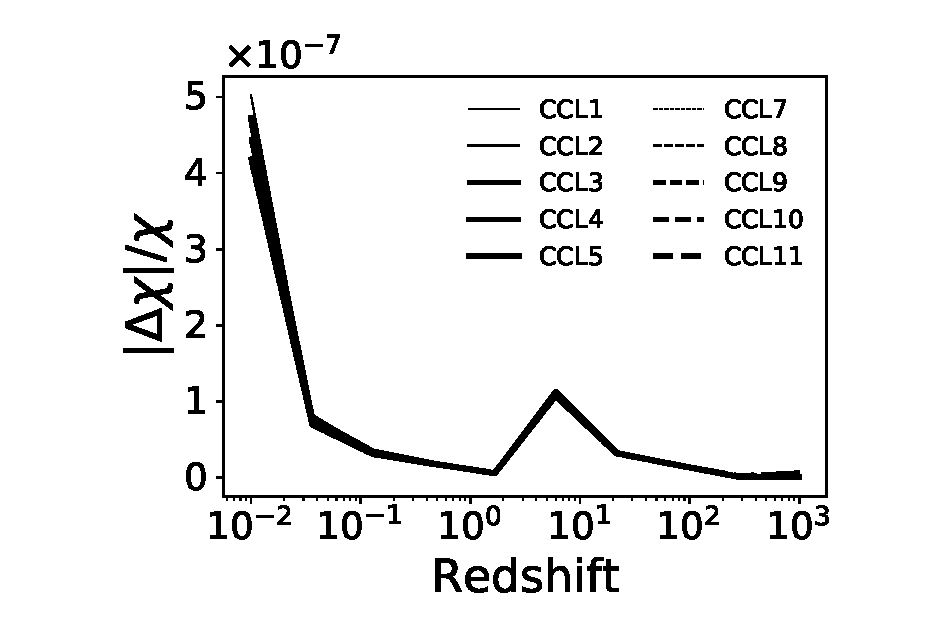
\includegraphics[width=0.45\textwidth]{distances.eps}
  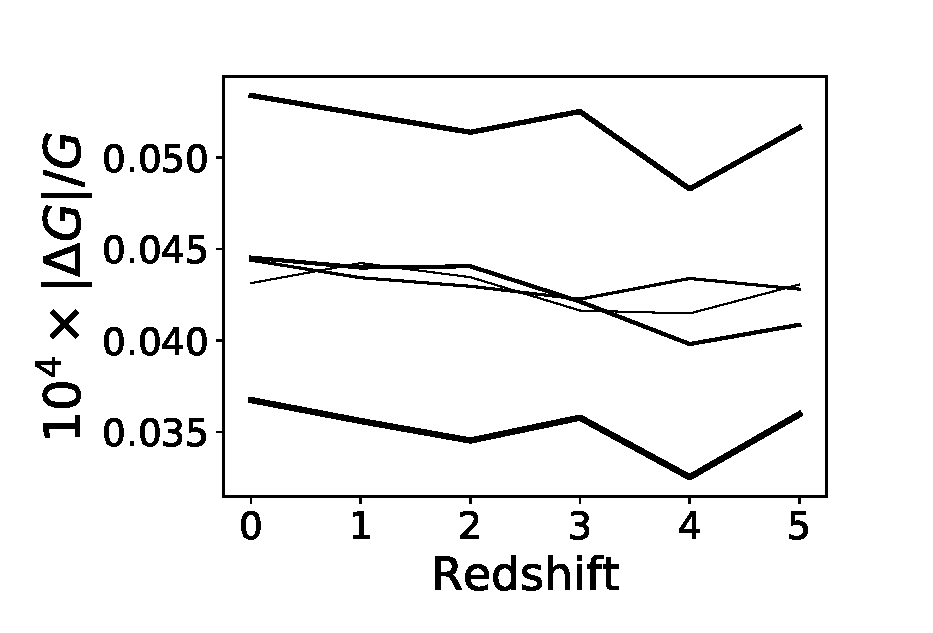
\includegraphics[width=0.45\textwidth]{growth.eps}

  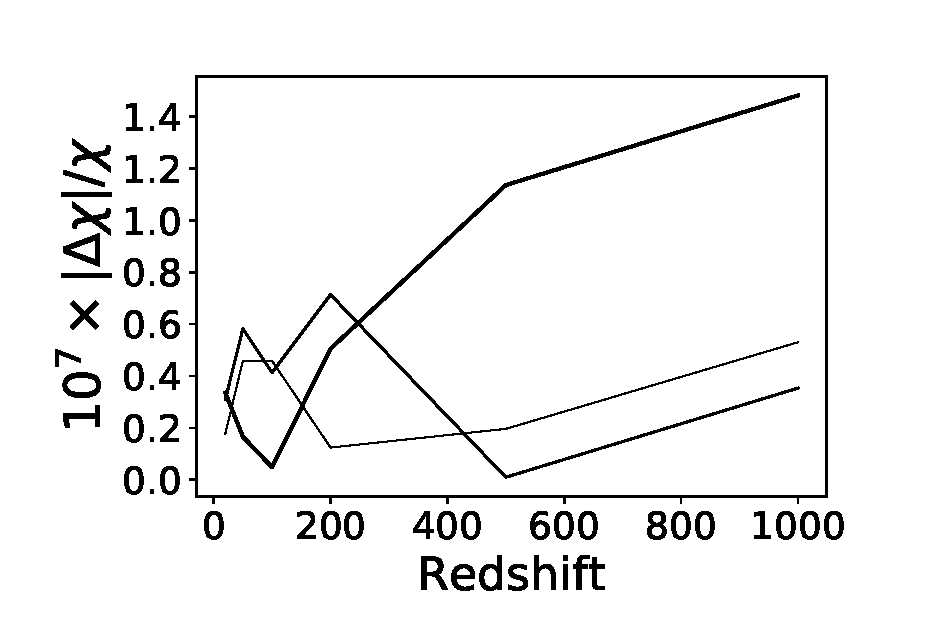
\includegraphics[width=0.45\textwidth]{distances_hiz.eps}
  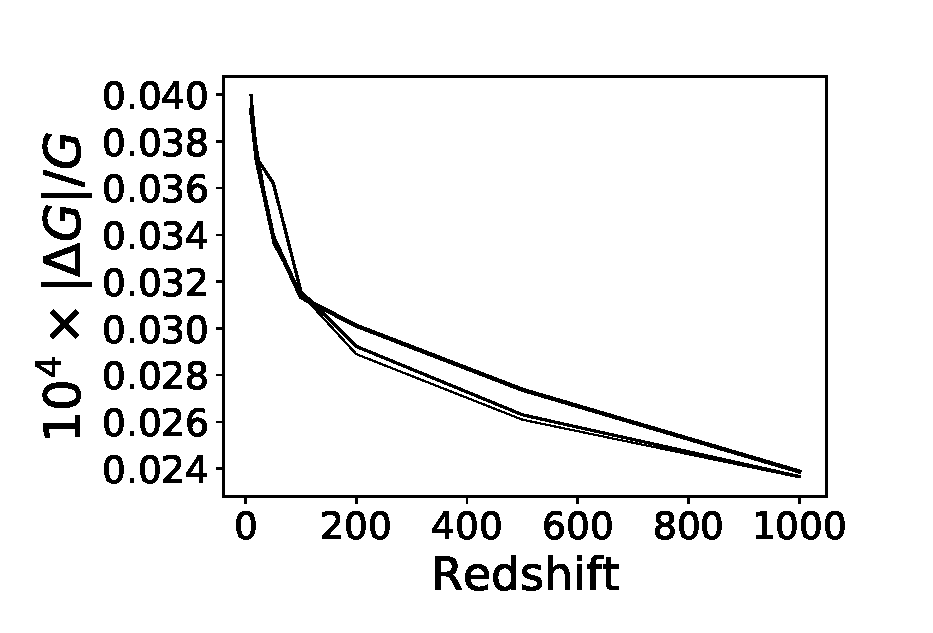
\includegraphics[width=0.45\textwidth]{growth_hiz.eps}
  \caption{Accuracy achieved by \ccl in the prediction of distances (left panels) and growth factor (right panels) for models CCL1-5 documented in Table \ref{tab:cosmologies}. Different models correspond to different thickness curves. The top panels represent the accuracy checks at low redshift, while the bottom panels demonstrate accuracy up to high redshift.}
  \label{fig:distancegrow}
\end{figure*}

\begin{table*}[t]
  \centering
  \begin{tabular}{ l c | c c c c c c c c c c }
    \hline
    \multicolumn{12}{|c|}{Cosmological models with massive neutrinos} \\
    \hline
    \hline
    Acronym & Model & $\Omega_m$ & $\Omega_b$ & $\Omega_\Lambda$ & $h_0$ & $\sigma_8$ & $n_s$ & $w_0$ & $w_a$ & $N_{eff}$ & $m_\nu$ (eV) \\
    \hline
    CCL7 & flat $\Lambda$CDM, $m_\nu$ & 0.3 & 0.05 & 0.7 & 0.7 & 0.8 & 0.96 & -1 & 0 & 3 & \{0.04, 0, 0\} \\
    CCL8 & $w_0$ $\Lambda$CDM, $m_\nu$ & 0.3 & 0.05 & 0.7 & 0.7 & 0.8 & 0.96 & -0.9 & 0 & 3 & \{0.05, 0.01, \} \\
    CCL9 & $w_a$ $\Lambda$CDM, $m_\nu$ & 0.3 & 0.05 & 0.7 & 0.7 & 0.8 & 0.96 & -0.9 & 0.1 & 3 & \{0.03, 0.02, 0.04\} \\
    CCL10 & open $w_a$ $\Lambda$CDM, $m_\nu$ & 0.3 & 0.05 & 0.65 & 0.7 & 0.8 & 0.96 & -0.9 & 0.1 & 3 & \{0.05, 0, 0\}  \\
    CCL11 & closed $w_a$ $\Lambda$CDM, $m_\nu$ & 0.3 & 0.05 & 0.75 & 0.7 & 0.8 & 0.96 & -0.9 & 0.1 & 3 &\{0.03, 0.02, 0\} \\
    \hline
  \end{tabular}
  \caption{Cosmological models with massive neutrinos used in testing \ccl against independently produced benchmarks}
  \label{tab:cosmologies_nu}
\end{table*}

\begin{figure*}
  \centering
  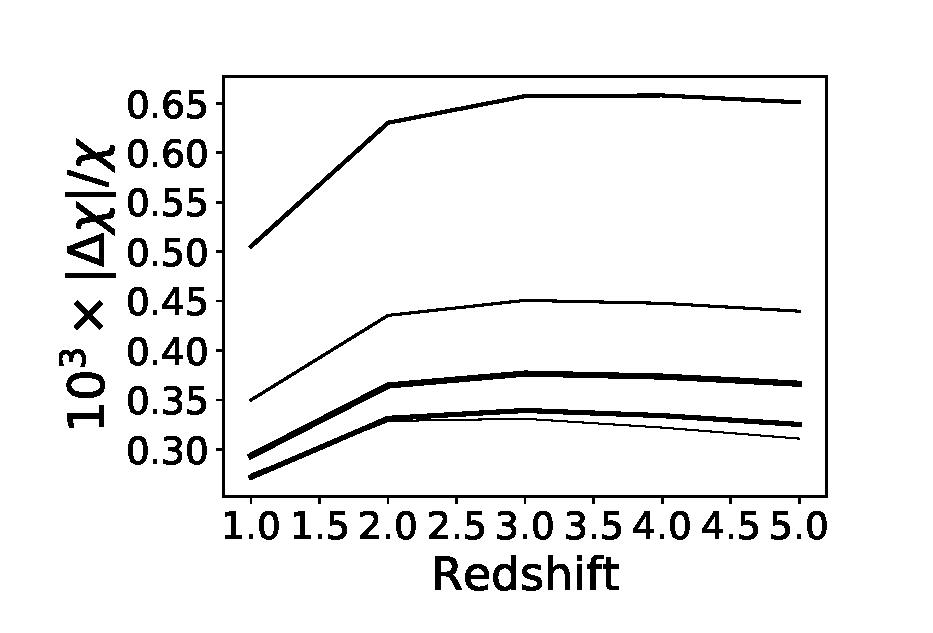
\includegraphics[width=0.45\textwidth]{distances_nu}
  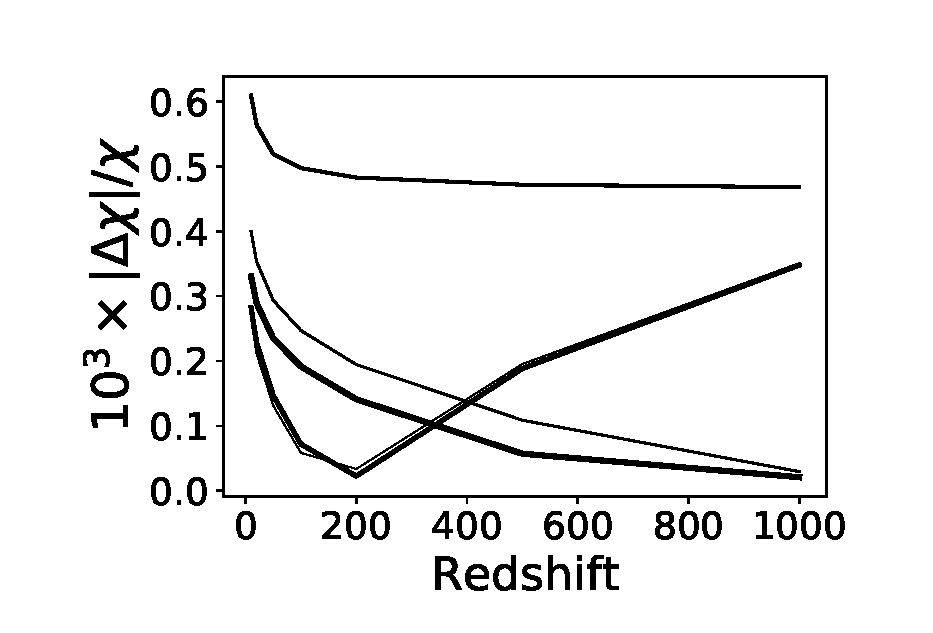
\includegraphics[width=0.45\textwidth]{distances_nu_hiz}
  \caption{Accuracy achieved by \ccl in the prediction of distances for models CCL7-11 with massive neutrinos, documented in Table \ref{tab:cosmologies_nu}. Different models correspond to different thickness curves. The left panel represent the accuracy checks at low redshift, while the right panel demonstrates accuracy up to high redshift. Note that we allow up to $10^{-3}$ fractional difference between benchmarks and \ccl in this case, because benchmarks utilize a fitting function for the neutrino phase space integral which is itself not accurate to $10^{-4}$.}
  \label{fig:distancegrow_nu}
\end{figure*}

\subsection{Matter power spectra}

\subsubsection{Analytic expressions}
\vol{Elisa Chisari}

As discussed in Section \ref{sec:matterps}, several power spectrum methods are implemented in \ccl. Two of them, the BBKS \citep{BBKS} and the Eisenstein \& Hu methods are implemented for validation purposes only and feed into the tests for observables such as angular power spectra and correlation functions, as we will see in subsequent sections. These two implementations have been validated against independent implementations. For BBKS, this test was performed at $0\leq z \leq 5$ in the wavenumber range $10^{-3} \leq k \leq 10 h/$Mpc with 10 bins per decade, and yielded an accuracy level of $10^{-4}$.
\footnote{We noticed that there are 2 typographical errors for the BBKS transfer function in ``Modern Cosmology'' \citep{DodelsonBook} compared to the original BBKS paper. The quadratic term should be $(16.1q)^2$ and the cubic term should be $(5.46q)^3$. The BBKS equation is correct in \citet{PeacockBook}. Using the wrong equation can give differences in the results above the $10^{-4}$ level.}
For the Eisenstein \& Hu matter power spectrum, we obtained similar accuracy at $z=0$ for the same wavenumbers. The cosmologies for which the tests were implemented are specified in Table \ref{tab:tests}.

The BCM implementation for the impact of baryons on the matter power spectrum, described in Section \ref{sec:matterps} is also analytical, and accurate to $10^{-12}$.

\subsubsection{Validation of interpolation schemes}
\vol{Elisa Chisari, Christiane Lorenz}

In its default configuration, \ccl adopts the HaloFit \citep{CLASS_halofit} implementation by interpolating {\tt CLASS} power spectra outputs to model the matter power spectrum. The computation of the power spectrum from {\tt CLASS} can be significantly sped up by interpolating the matter power spectra in the range {\tt K$\_$MIN}~$<k<$~{\tt K$\_$MAX$\_$SPLINE} and extrapolating beyond it, as described in Section \ref{sec:implement}. In this section, we describe the loss of accuracy due to this method. The tests presented are performed in a flat $\Lambda$CDM cosmology with $\Omega_c=0.25$, $\Omega_b=0.05$, $A_s=2.1\times10^{-9}$, $h=0.7$ and $n_s=0.96$.

The accuracy of this approximation is shown in Figure \ref{fig:NLextrapol} for redshifts $z=0$, $z=3$ and $z=20$. We compare the nonlinear matter power spectrum at these redshifts, computed with the previously described approximation, to the matter power spectrum obtained by setting the power spectrum splines to high-accuracy values. We find that for typical values of $\Delta \ln k=10^{-2}$ and {\tt K$\_$MAX$\_$SPLINE}$=50$/Mpc, $\ln P$ has converged to an accuracy that surpasses the expected impact of baryonic effects on the matter power spectrum at $k>10/$Mpc.  (For an estimate of the impact of baryons on the total matter power spectrum, see \citealt{Schneider15}.) 

%------------------------
\begin{figure*}
\centering
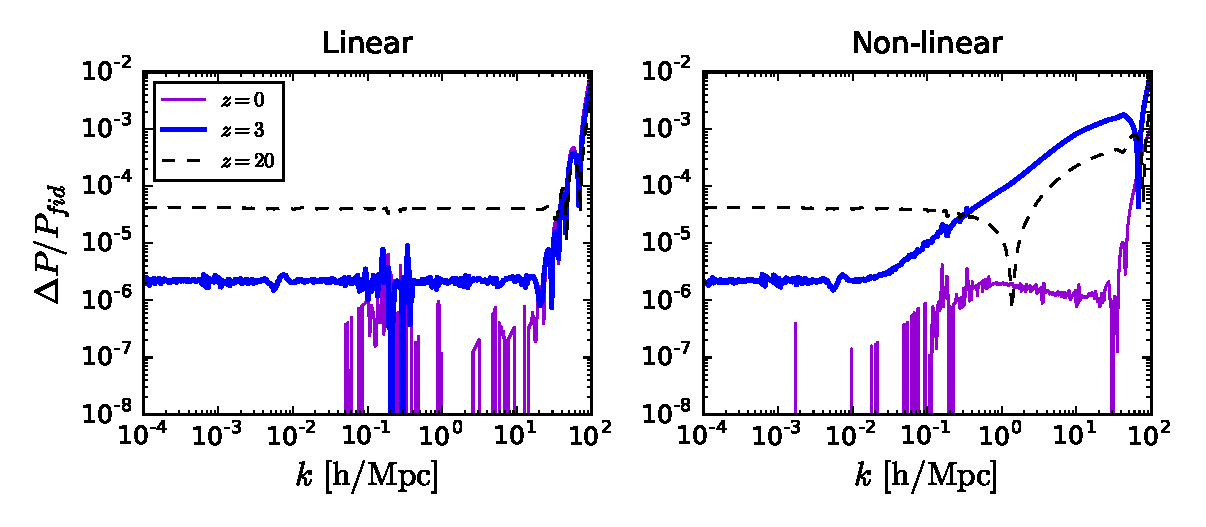
\includegraphics[width=1.0\textwidth]{plot_power.eps}
\caption{The relative error compared to power spectra produced with high values of the power spectrum splines, $P_{fid}$, produced by splining the matter power spectrum up to {\tt K$\_$MAX$\_$SPLINE} and extrapolating beyond this value with a second order Taylor expansion the natural logarithm of the matter power spectrum. The left panel shows the relative errors for the linear matter power spectrum at $z=0$, $z=3$ and $z=20$. The right panel shows the results for the non-linear matter power spectrum at the same redshifts. The standard \ccl parameters adopted are those corresponding to the black dashed curve. For comparison, the impact of baryonic physics on the matter power spectrum is $\sim 10\%$ at $k=1$/Mpc \citep{Schneider15}.}
\label{fig:NLextrapol}
\end{figure*}
%------------------------

With the implementation described above, the power spectrum splines are initialized up to {\tt K$\_$MAX$\_$SPLINE}. This is also true for the linear matter power spectrum, which is used within \ccl in particular to obtain $\sigma_8$ (see Eq. \ref{eq:sigR}). We have tested how this procedure affects the convergence of the linear matter power spectrum. We compare the fiducial \ccl output to the case where we set {\tt K$\_$MAX$\_$SPLINE}~$=5\times 10^3/$Mpc. The result is shown in Figure \ref{fig:NLextrapol}. For some applications that use the linear power spectrum, the user might need to increase the value of {\tt K$\_$MAX$\_$SPLINE}. While \ccl adopts certain fiducial values of the number of scale factor and wavenumber values to use in the interpolation, we have tested that increasing the sampling does not change the results presented in Figures \ref{fig:NLextrapol}.

In addition to the above tests in $\Lambda$CDM cosmologies without massive neutrinos, we have checked the impact of using splines at low and high $k$ in cosmologies CCL7, CCL8, and CCL9 with massive neutrinos, defined in Table \ref{tab:cosmologies_nu}. We compare the linear and nonlinear matter power spectrum as computed directly via {\tt CLASS} to that computed using {\tt CLASS} via \ccl (i.e. using splines at high and low k). We find that for $k$  between {\tt K$\_$MIN} and {\tt K$\_$MIN$\_$SPLINE}, the two power spectra agree to better than $10^{-4}$ in all models. For $k$ between {\tt K$\_$MAX$\_$SPLINE} and {\tt K$\_$MAX}, agreement is better than $10^{-3}$, which we deem sufficient given the significant uncertainties introduced at these small scales, e.g. baryonic effects. The fractional difference between the two nonlinear power spectra is plotted in Figure \ref{fig:power_nu}. 

\begin{figure}
\centering
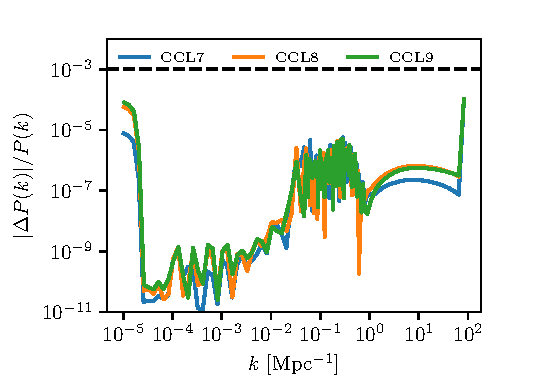
\includegraphics[width=0.47\textwidth]{pk_class_nu_NL}
\caption{Fractional difference between the nonlinear matter power spectrum as computed directly via {\tt CLASS} with that computed using {\tt CLASS} via \ccl in cosmologies CCL7, CCL8, and CCL9 with massive neutrinos.}
\label{fig:power_nu}
\end{figure}

%-------------------------------------------------------------------------------
\subsubsection{Generalized validation of the power spectrum over $\Lambda$CDM parameter space}
\vol{Phil Bull}
\cont{ `Fair' sampling of parameter space with Latin Hypercubes. Summary statistics used, and binning of power spectrum in $k$ and $z$. Precision settings used for CLASS. Estimates of run-time. Results. Range of validity.}

\todo{Have the undergraduate students who did most of this work been included as authors on the paper? - DL}

While concentrating on individual points in cosmological parameter space allows us to perform detailed validation tests, as above, it is important for \ccl to also be validated across a wide range of cosmological parameter values, e.g. to ensure validity for MCMC analyses. In this section, we present a set of validation tests for the \ccl linear and non-linear matter power spectrum functions that spans a broad range of $\Lambda$CDM parameters.

Covering a full range of all 5 $\Lambda$CDM parameters on a regular grid would be prohibitively expensive, so an alternative method for fairly (but more sparsely) sampling the parameter space is needed. We use Latin Hypercube Sampling to determine a tractably-sized set of sample points. This splits the parameter space into a regular grid with a given number of cells per dimension. The sample points are then chosen by going through each dimension in turn and choosing a cell at random {\it without replacement}, so that a given cell of a given dimension is only ever chosen once. This is repeated until all cells in all dimensions contain a single sample. This has the effect of covering the space uniformly but sparsely. The exact location of the sample within each cell can be chosen from a uniform distribution within that cell, but for simplicity we put each sample at the cell centre. The ranges used for each parameter are shown in Table~\ref{tab:paramranges}.
%
\input{param_ranges_varric}

For each set of parameters, we then calculate the linear and non-linear power spectra using \ccl for a range of redshifts ($z \in \{ 0,\, 0.5,\, 1,\, 1.5,\, 2,\, 2.5\}$) and wavenumbers ($k \in [10^{-4}, 10^0]$ Mpc$^{-1}$). A corresponding set of reference power spectra is then produced using {\tt CLASS}, which we run with settings chosen to produce high-precision results, taken from the {\tt pk\_ref.pre} precision file that is bundled with {\tt CLASS}.

To quantify the level of agreement between the \ccl and reference power spectra, we use the following summary statistic that can be summed over a chosen set of bins in redshift and wavenumber:
\begin{equation}
\Delta = \sum_{ij} \Theta \left ( \log_{10} \left | \frac{P_{\rm CCL}(k_i, z_j) - P_{\rm ref}(k_i, z_j)}{P_{\rm ref}(k_i, z_j) \Delta_{\rm thres}} \right | \right ).
\end{equation}
Here, $\Delta_{\rm thres}$ is a target threshold for the fractional deviation between the power spectra, and we have defined $\Theta(x) \equiv x ~~(x \ge 0)$ and $0$ otherwise. Bins where the \ccl power spectrum deviates from the reference power spectrum by a fraction less than $\Delta_{\rm thres}$ do not contribute to the statistic, so the aim is to have $\Delta = 0$ (i.e. no deviation beyond the threshold in any bin). If deviations are found, however, they are weighted logarithmically -- one large deviation of several orders of magnitude affects the statistic as much as a few smaller deviations of order $\sim \Delta_{\rm thres}$.
\todo{This section still needs discussion and conclusions, right? -DL}

\subsubsection{Validation of the Cosmic Emulator implementation}
\vol{Elisa Chisari}
\todo{I think this section should go before the one on generalized validation of the power spectrum over LCDM space, because that one refers to 'the sections above' as being at specific cosmologies, which is the case here. - DL}\todo{The only caveat is that the generalized validation scheme doesnt account for the emulator - EC.}
\citet{Lawrence17} quantified the accuracy of the matter power spectrum from their emulation scheme by comparing their predictions to the resulting power spectra from the numerical simulations used for the calibration of their scheme. We repeated this procedure making the emulator predictions via \ccl for a subset of emulator cosmologies. 

Our results, presented in the form of absolute fractional accuracy of the power spectra, are shown in Figure \ref{fig:emuacc}. For cosmologies without neutrinos, we required the matter power spectrum at $z=0$ to be within $1\%$ of the smoothed simulated power spectrum from \citet{Lawrence17} (see their Figure 6). Similarly, we required $3\%$ accuracy for cosmologies with neutrinos (their Figure 5). The cosmologies that were tested are the ones listed in Table \ref{tab:cosmologies}, which are described in detail in \citet{Lawrence17}.

\begin{figure*}
  \centering
  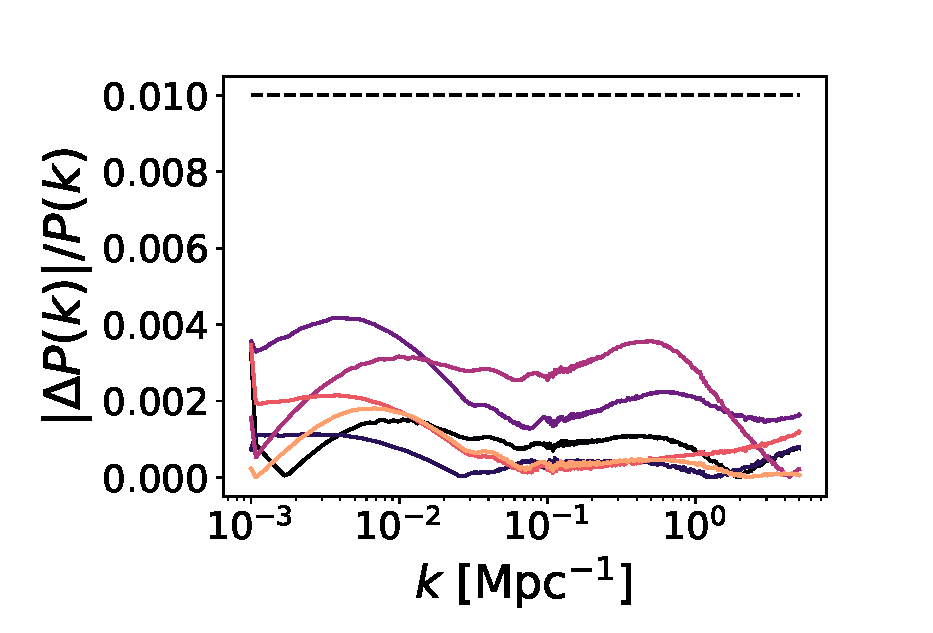
\includegraphics[width=0.45\textwidth]{poweremu.eps}
  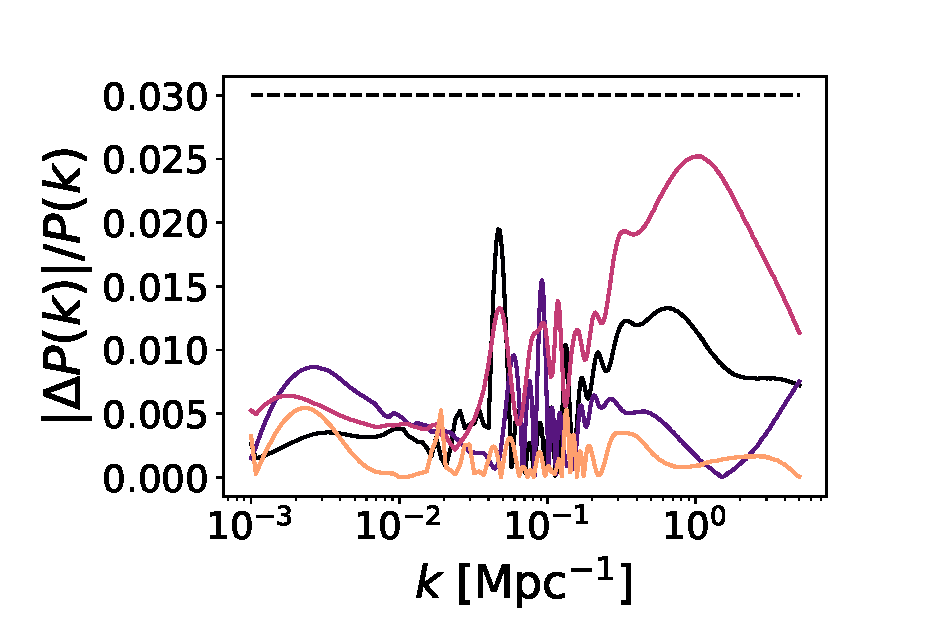
\includegraphics[width=0.45\textwidth]{poweremu_nu.eps}
  \caption{Absolute fractional accuracy in the matter power spectra obtained by calling the cosmic emulator from \ccl and the smoothed simulated spectra from \citep{Lawrence17}. The left panel shows the results for cosmologies without neutrinos; the right panel, results for cosmologies with neutrinos.}
  \label{fig:emuacc}
\end{figure*}

\subsection{Halo bias and halo mass function}

Independent codes were utilized to test the accuracy of halo mass function predictions. These predictions are computed from power spectra obtained using the BBKS approximation. For the halo mass function, we compare the value of $\sigma$, $\log(\sigma^{-1})$, and the value of the halo mass function in the form used in \cite{Tinker2008},
\begin{equation}
\log[(M^2/\bar{\rho}_m)dn/dM].
\end{equation}
We note that while we maintain the $10^{-4}$ for our evaluations of $\sigma$, the accuracy degrades to a value of $5\times10^{-3}$ for the halo mass function evaluation, primarily at the high halo mass and high redshift domains. We find that this increased error is acceptable, as the level of precision is significantly better than the accuracy of current halo mass function models. This is demonstrated in Figure~\ref{fig:hmf}, where this calculation has been run for a single cosmology using the Tinker 2010 halo mass function. While there is a degradation in accuracy due to our current spline treatment of the log inverse of $\sigma(M)$, we note that it does not significantly degrade our halo mass function determination. While improvement on this remains a task for the future, the halo mass function varies between fitting functions significantly more than this remaining error. As of this time, we currently do not have independent benchmarks for the halo bias function, though it should be noted that this calculation does not involve any additional functions beyond $\sigma(M)$ and should hold to the $10^{-4}$ tolerance level.

\begin{figure*}
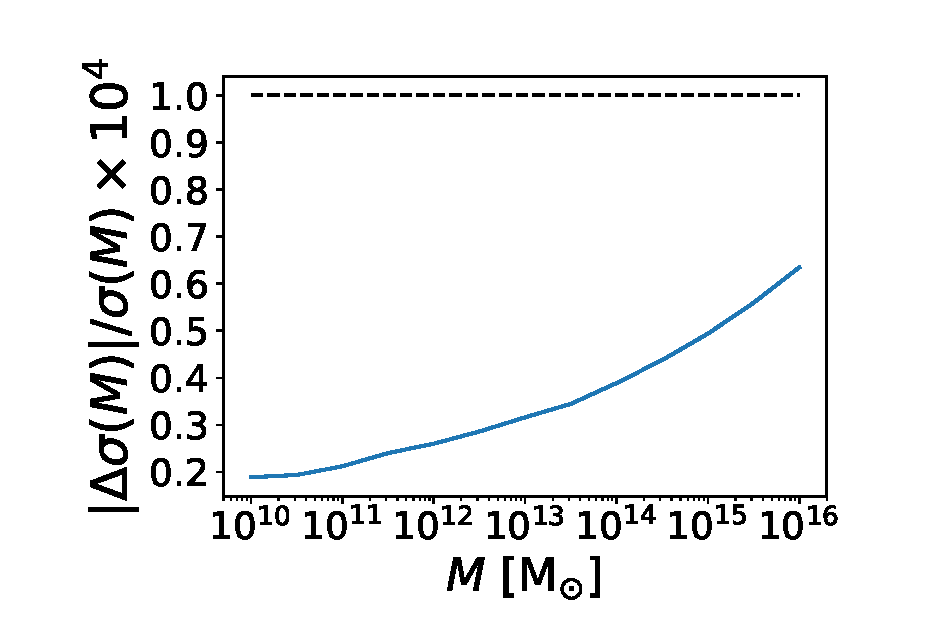
\includegraphics[width=0.32\textwidth]{hmf_model1.eps}
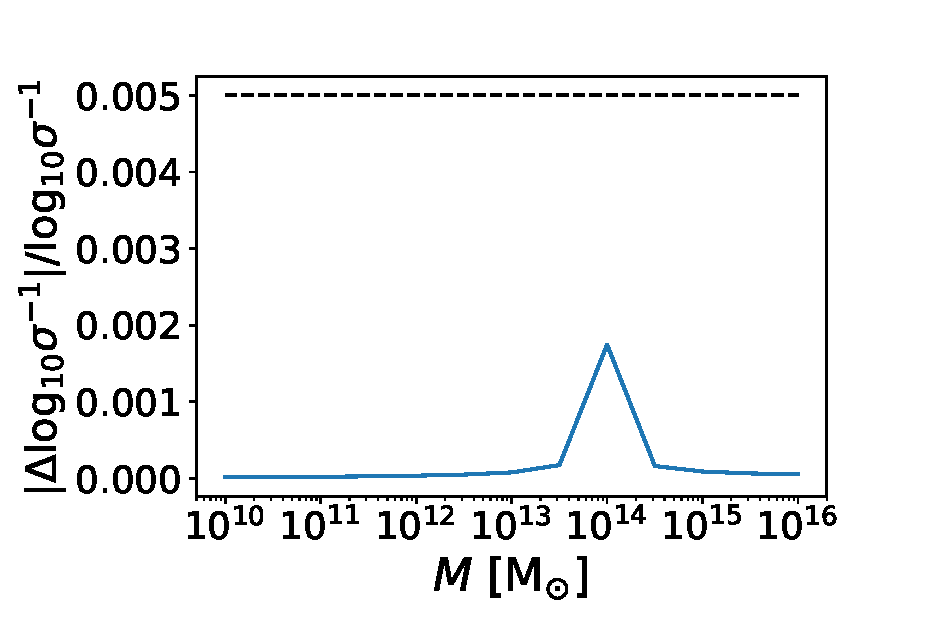
\includegraphics[width=0.32\textwidth]{hmf_model1_b.eps}
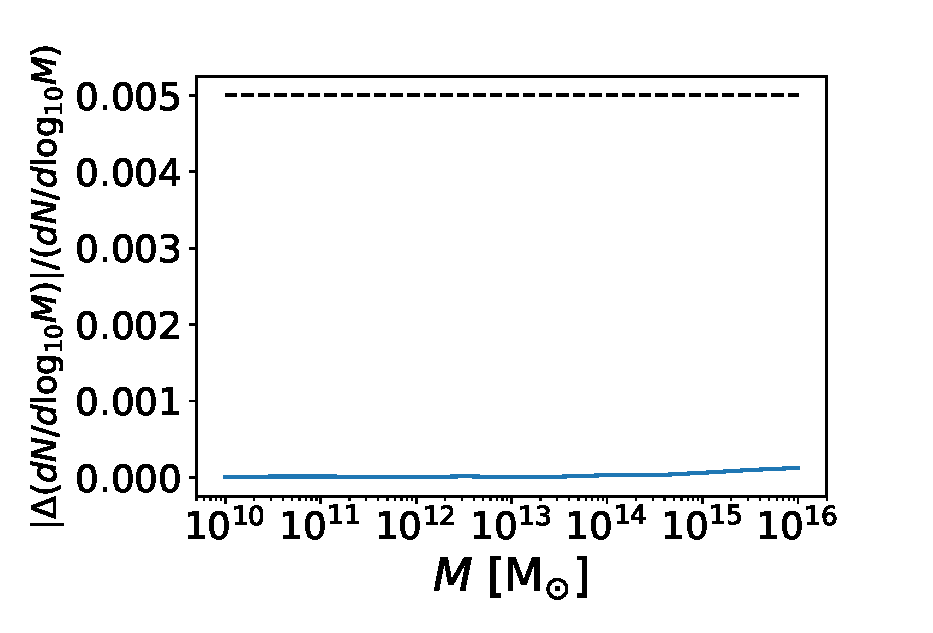
\includegraphics[width=0.32\textwidth]{hmf_model1_c.eps}
\caption{Three different numerical tests of the halo mass function calculation. In each line, the blue line is the fractional error in the function, while the black dashed line represents our error tolerance. The first panel demonstrates the robust calculation of $\sigma(M)$. The second panel demonstrates a numerical quirk in our spline treatment that is currently not addressed, but does reduce the numerical accuracy in returning the log inverse of $\sigma(M)$. We note that this does not significantly impact the error in the halo mass function in the final panel.}
\label{fig:hmf}
\end{figure*}

\subsection{Two-point statistics}

We used the BBKS linear matter power spectrum to compare two-point statistics for two redshift bins, resulting in three tomography combinations, ($1-1$),($1-2$),($2-2$). We computed the following quantities:
\begin{itemize}
\item Number counts angular power spectra: density term only (no magnification, RSD, etc.) with non-evolving linear bias $b(z) = 1$, in the range $10 < \ell < 10000$, using $5$ bins per decade,
\item Lensing convergence angular power spectra: leading order convergence term only (no magnification or intrinsic alignments), in the same range and with the same resolution as the case above,
\item Number counts angular correlation functions in the range $0.01 \deg < \theta < 5 \deg$, using 5 bins per decade, and
\item Lensing shear angular correlation functions ($\xi_+$,$\xi_-$), similarly to above.
\end{itemize}
We adopted the following analytic redshift distributions: a Gaussian with $\sigma = 0.15$, centered at $z_1 = 1$; and another Gaussian with the same dispersion but centered at $z_2 = 1.5$. We repeated the exercise for two redshift distribution histograms shown in Figure \ref{fig:zhistos}. Besides these two-point functions, we also validated the computation of the CMB lensing power spectrum, using the same $\ell$ binning described above. 

%------------------------
\begin{figure}
\centering
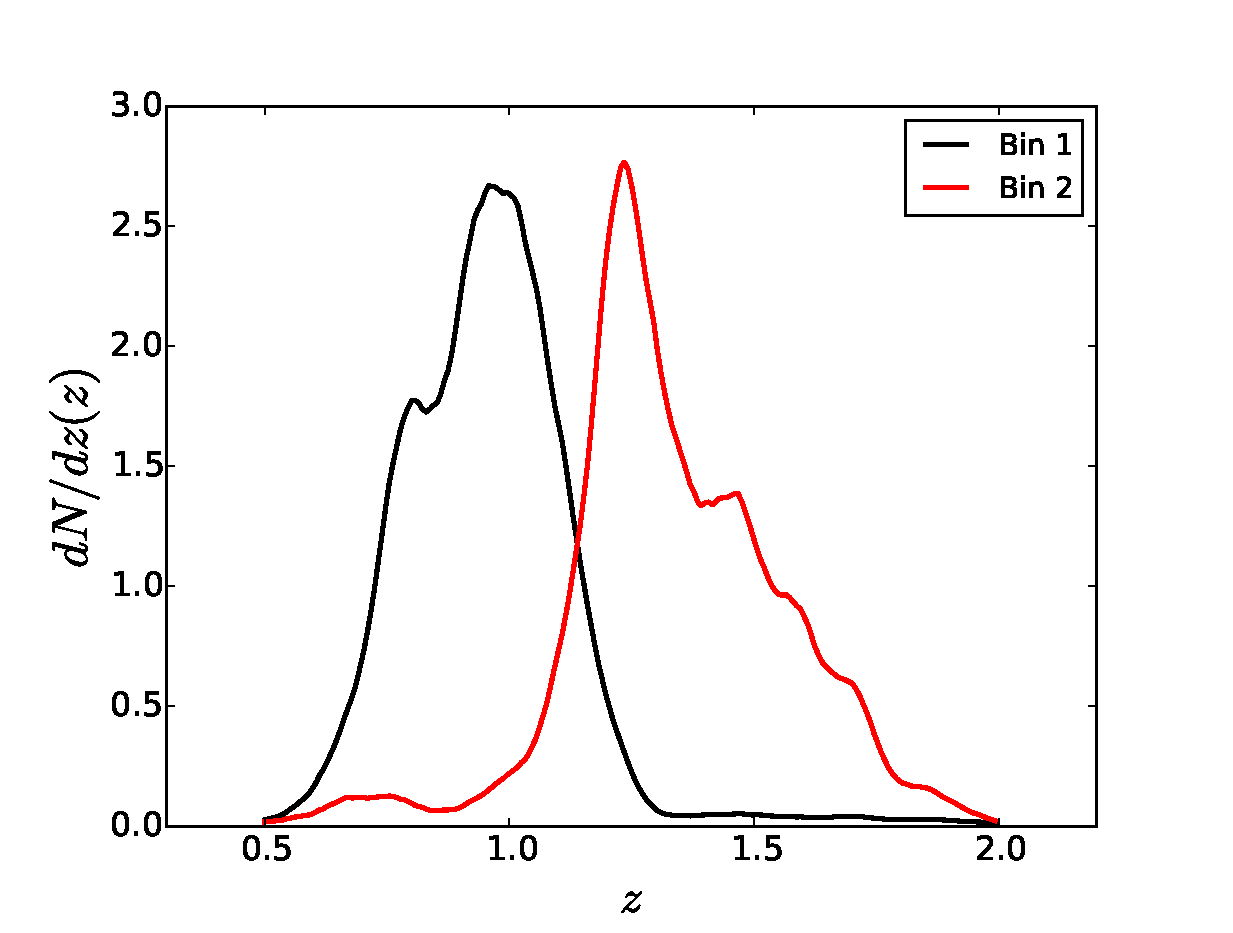
\includegraphics[width=0.47\textwidth]{zdist.eps}
\caption{Binned redshift distributions used for code comparison project.}
\label{fig:zhistos}
\end{figure}
%------------------------

\begin{figure*}
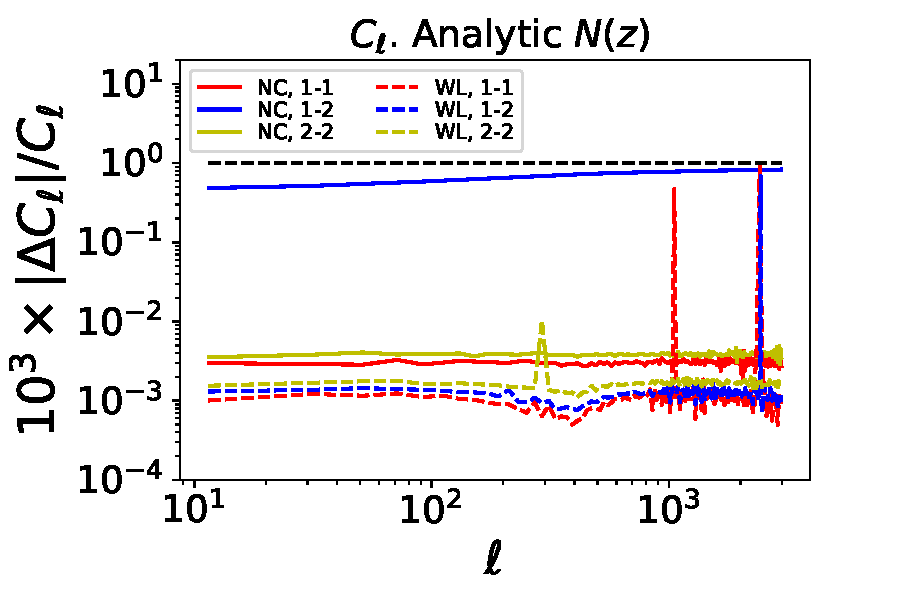
\includegraphics[width=0.49\textwidth]{Cl_analytic}
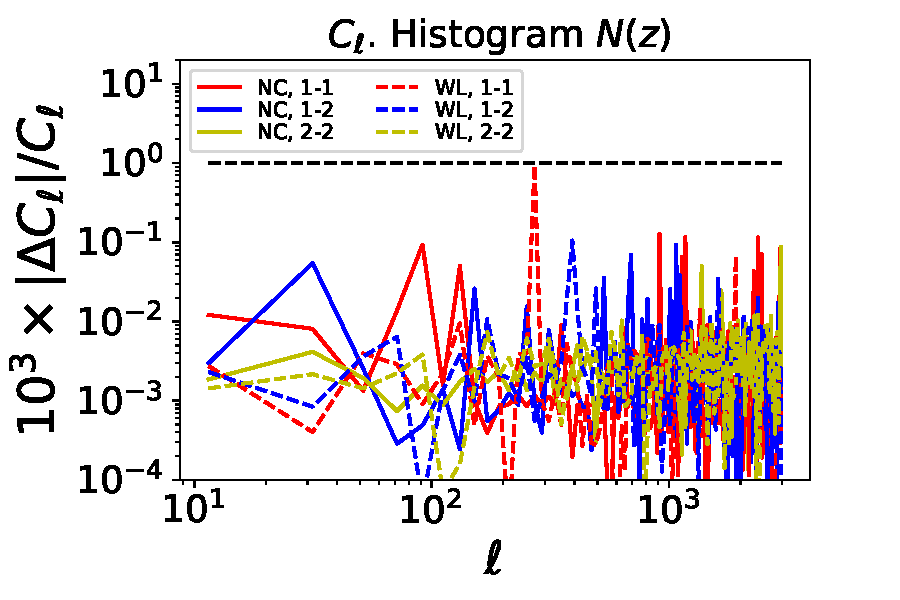
\includegraphics[width=0.49\textwidth]{Cl_histo}
\caption{Tests of the angular power spectrum accuracy. Benchmark comparisons for number counts (solid) and weak lensing (dashed) power spectra are shown for analytic and histogram-based redshift distributions in the left and right panels respectively.}
\label{fig:cls_limber}
\end{figure*}
\begin{figure}
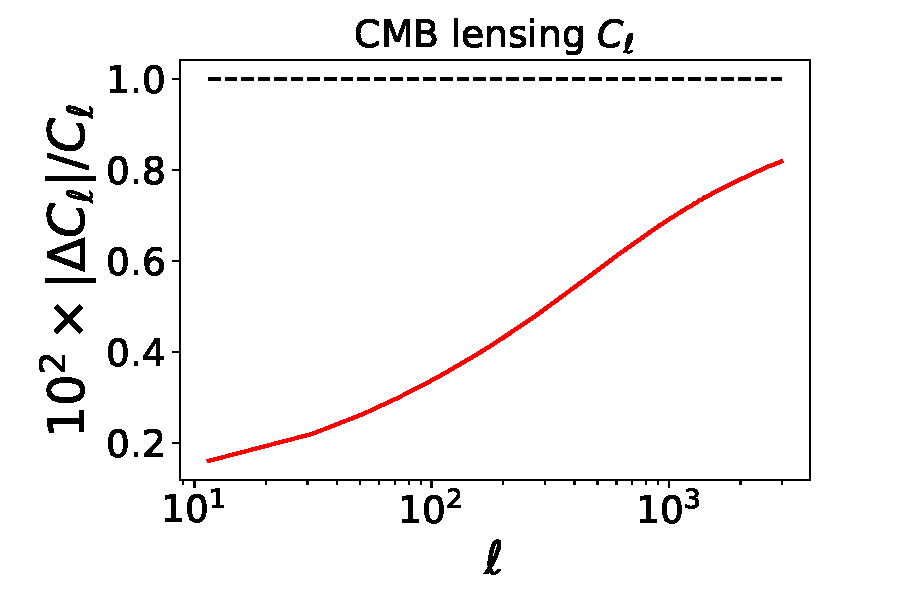
\includegraphics[width=0.49\textwidth]{Cl_cmblens}
\caption{Same as Fig. \ref{fig:cls_limber} for the CMB lensing power spectrum.}
\label{fig:cls_cmblens}
\end{figure}

For $C_\ell$ computations, we achieved a relative difference between \ccl and the benchmarks of $<10^{-3}$. This applied both to analytic redshift distributions and histograms, for auto- and cross-correlations between bins for both galaxy clustering and weak lensing, as shown in Figure \ref{fig:cls_limber}. The CMB lensing result is shown in Figure \ref{fig:cls_cmblens}.


To obtain realistic targets for the convergence of projected correlation function computations for LSST analyses, we calculated the expected statistical uncertainty of the clustering and lensing correlation functions of the LSST gold sample \todo{Add reference} assuming an effective source galaxy density of $n_\mathrm{eff} = 26\,\mathrm{gal/sq\,arcmin}$ for galaxy shape distortions, and galaxy density of $n_\mathrm{gold} = 45\,\mathrm{gal/sq\,arcmin}$ for number counts. Specifically, we calculated the Gaussian covariance of angular correlation functions following the formalism of \citet{2008A&A...477...43J}, and note that leaving out the non-Gaussian covariance terms makes our accuracy criterion more conservative. We split the galaxy samples into 10 tomography bins, defined to contain equal numbers of galaxies. The accuracy test then proceeded as follows. We compared the difference between \ccl calculated lensing and clustering correlations and the benchmarks, for the analytic redshift distributions and for auto-correlations of redshift bins only. To pass the benchmark test, we required that this difference be smaller than half of the value of the error bar derived from the covariance for each correlation function computed. Specifically, we took the value of the covariance in the bins centered at $z=1$ and $z=1.5$ to compare to the benchmarks.

The results of this validation procedure for the projected correlation function are shown in Figure \ref{fig:corrval}. Our results suggest that the convergence between \ccl predictions and benchmarks is below the expected statitical uncertainty. 

\begin{figure*}
\centering
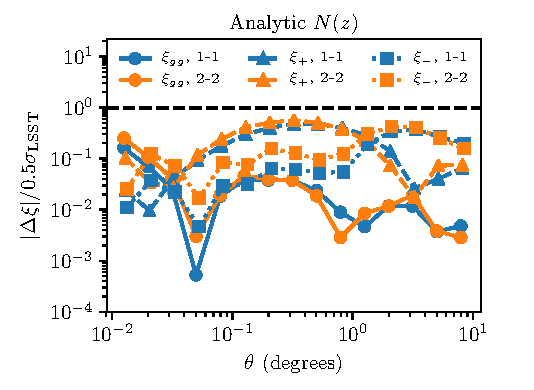
\includegraphics[width=0.47\textwidth]{projected_correlation_error_comparison_analytic} 
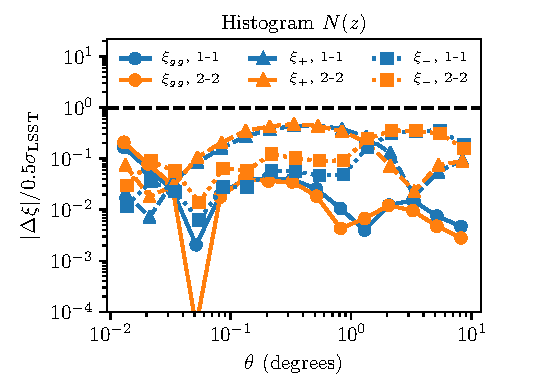
\includegraphics[width=0.47\textwidth]{projected_correlation_error_comparison_histo} 
\caption{Comparison between the predicted projected correlation functions and the expected uncertainties for LSST. The left panel shows predictions for the analytic redshift distrobutions, while the right panel shows the case of the redshift histograms. The different markers and colors indicate clustering ($w_{gg}$, filled circles) or lensing ($\xi_{\pm}$, filled triangles and squares) auto-correlations of the $1$-$1$ or $2$-$2$ redshift bin combinations.}
\label{fig:corrval}
\end{figure*}

  
The 3-dimensional spatial correlation function $\xi(r)$ was validated by comparing with an independent, precise numerical transform. We calculated $\xi(r)$ 
by transforming the \ccl non-linear HaloFit power spectrum using this independent code for the five cosmologies listed in Table~\ref{tab:cosmologies} at 
redshifts $z = 0,1,2,3,4,5$.  We then compared with the $\xi(r)$ from \ccl with a sampling of $P(k)$ 
equal to {\tt N$\_$K$\_$3DCOR} bins per decade. The default value of {\tt N$\_$K$\_$3DCOR}~=~100,000 results in a relative agreement 
at the level of $\Delta \xi(r) / \xi(r) < 2.5 \times 10^{-3}$ for $0.1 < r < 250$~Mpc and $z=0$. The agreement was better for higher redshifts.
We also compared the absolute value of $r^2 \xi(r)$ and find a maximum difference of $\Delta (r^2 \xi(r)) < 3.0 \times 10^{-2}$ for the range 
$r = 0.1 - 250$~Mpc. This corresponds to approximately $0.08\%$ of the Baryon Acoustic Oscillation peak value of $r^2 \xi(r)$. At the peak, the difference is only $9.0 \times 10^{-3}$, or 0.024\% of the peak height. The results are shown in Fig.~\ref{fig:benchmark_xi}
%
\begin{figure*}
\centering
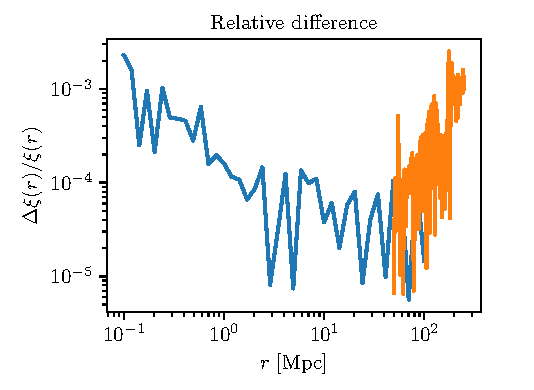
\includegraphics[width=0.47\textwidth]{benchmark_xi_rel} ~~~
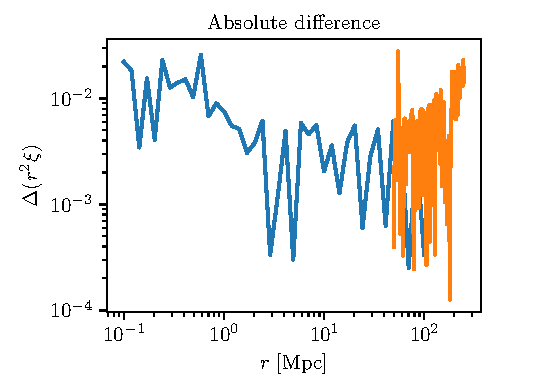
\includegraphics[width=0.47\textwidth]{benchmark_xi_abs} 
\caption{Comparison of the CCL calculation of the three-dimensional spatial correlation function $\xi(r)$ with a precise, numerical transform of the \ccl non-linear Halofit power spectrum. The left panel shows the relative error $\Delta \xi(r) / \xi(r)$. The right panel shows the absolute error in $r^2 \xi(r)$. Both panels are for the $w_a$~LCDM model of Table~\ref{table:code_comp} at redshift zero. \mi{John: Which models: there seems to be a typo.}}
\label{fig:benchmark_xi}
\end{figure*}
%

To further validate the $P(k) \to \xi(r)$ transform we performed a test using an analytical function $\xi(r) = (r / r_0)^a$, whose inverse transform $P(k)$ 
has a known analytic form. We used $r_0 = 5 h^{-1}$~Mpc$^{-1}$ and $a = -1.67$, which approximates the actual three-dimensional correlation function.   
We then compared the \ccl calculation of $\xi(r)$ to the known analytic result. The relative difference $\Delta \xi(r) / \xi(r)$ was found to be   
less than 0.4\% in the range $1 < r < 200$~Mpc rising to about 5\% at $r = 1000$~Mpc (see Fig.~\ref{fig:analytic_xi}). For $r=0.1-0.8$~Mpc the relative difference is $\approx$8\%. The accuracy at low and high distances can be improved by increasing the range over which the power spectrum splines are evaluated.
%
\begin{figure*}[htbp]
\centering
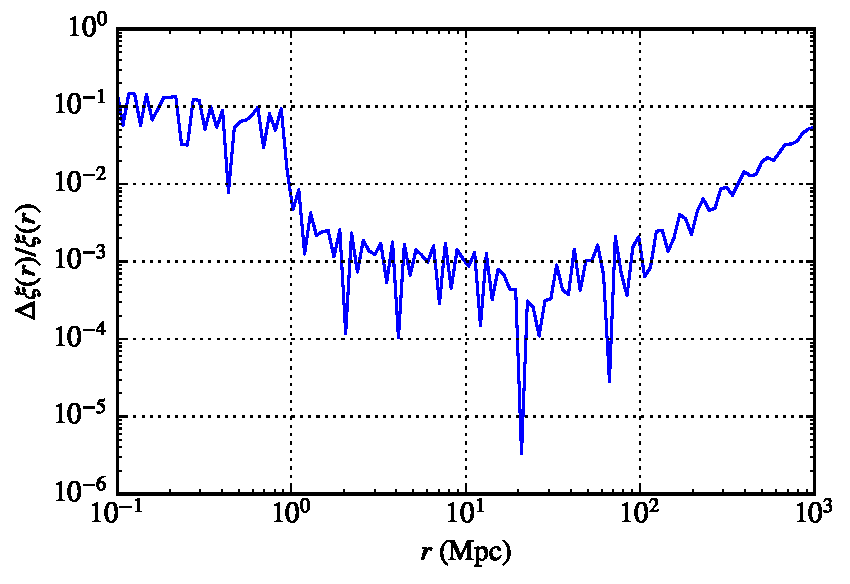
\includegraphics[width=0.47\textwidth]{analytic_xi}
\caption{The relative error in the three-dimensional spatial correlation function computed using the CCL algorithm compared to an analytic function $\xi(r) = (r/r_0)^a$ whose inverse transform $P(k)$ is known analytically. In this validation test, the known $P(k)$ was transformed with the \ccl algorithm and compared to the known analytic result for $\xi(r)$.}
\label{fig:analytic_xi}
\end{figure*}

\subsubsection{\tt Angpow}

\ccl performs non-Limber computations of angular power spectra through the {\tt Angpow} library as detailed in Section \ref{sec:angpow}. The \texttt{Angpow} software was tested against \texttt{CLASS} and the native \ccl computation and can perform the same computations approximately an order of magnitude faster ($\mathcal{O}(1s)$). 
Its precision and speed parameters were optimised so that the relative numerical error compared with a high precision computation is two orders of magnitude below the relative cosmic variance $\sqrt{2/(2\ell+1)}$, from $\ell=2$ to $\ell=1000$. We demonstrate this in Figure \ref{fig:angpow}, where we plot the angular clustering power spectrum for a sample of galaxies with $\langle z \rangle=1$ and a Gaussian redshift distribution that extends between $|z-\langle z \rangle|z<5\sigma_z$, where $\sigma_z=0.02$, for a CCL6 cosmology. 
The non-Limber prediction deviates from the Limber case at low $l$ as expected. The right panel shows the fractional difference between the non-Limber curves and the Limber case, demonstrating the accuracy of the {\tt Angpow} prediction for our choice of precision and speed parameters. 
Also the native non-Limber computation and {\tt Angpow} were tested to recover the Limber approximated curve at high $\ell$ for a wide Gaussian window ($\sigma_z=0.1$). The relative errors with respect to the Limber result at high $\ell$ are below two orders of magnitudes with respect to cosmic variance. 

\begin{figure*}[htbp]
\centering
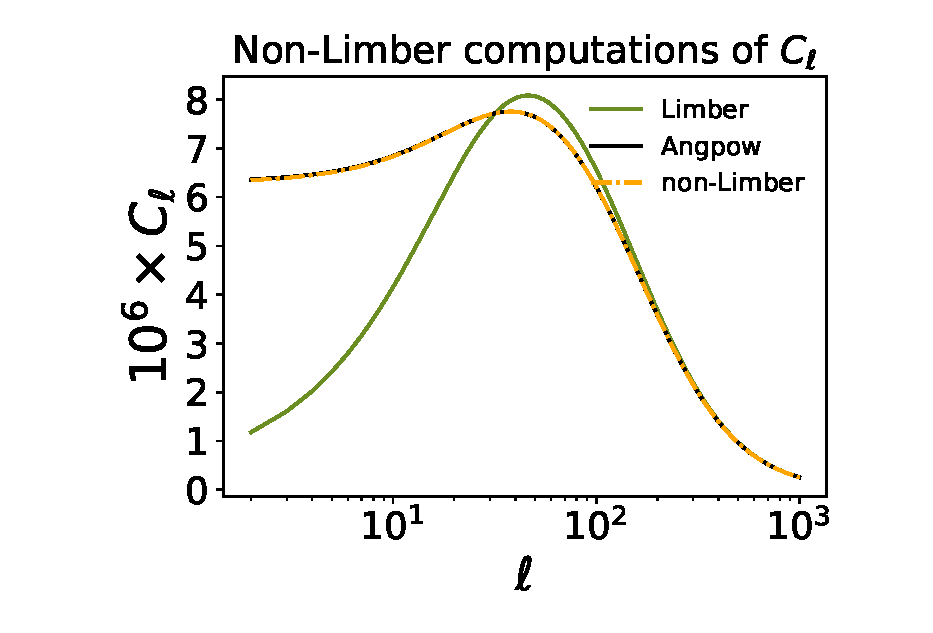
\includegraphics[width=0.47\textwidth]{angpow1}
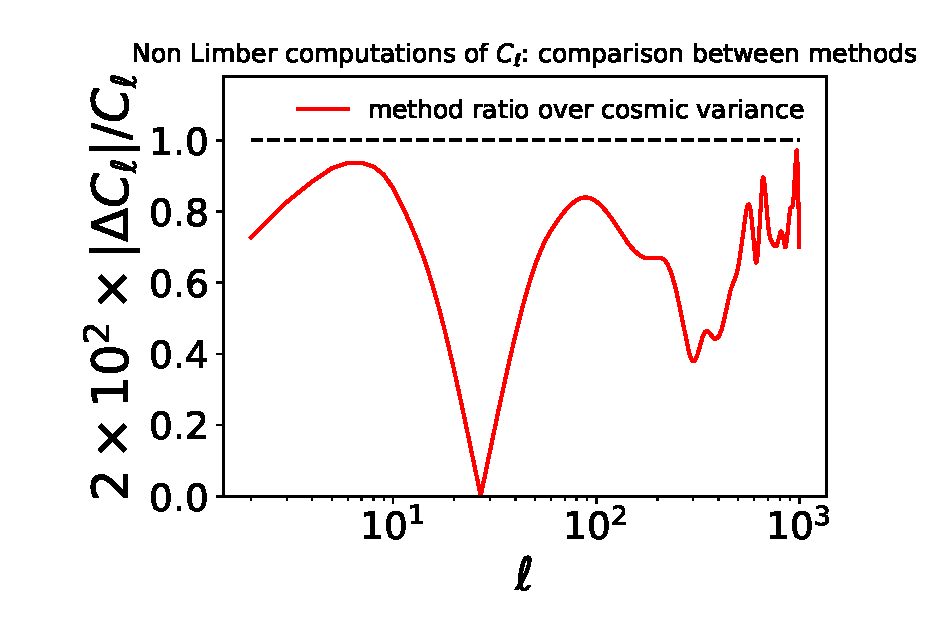
\includegraphics[width=0.47\textwidth]{angpow3}
\caption{Different predictions for the clustering angular power spectrum of a sample of galaxies with a Gaussian redshift distribution centered on $\langle z \rangle =1$. The left panel shows the $C_l$ predictions from the Limber case (green), the non-Limber case native to \ccl (yellow dot-dashed) and {\tt Angpow} (black). The right panel shows the fractional difference in the predicted clustering angular power spectrum between {\tt Angpow} and the native \ccl non-Limber computation. The relative numerical error compared with a high precision computation is two orders of magnitude below the relative cosmic variance: $\sqrt{2/(2\ell+1)}$.\todo{Fix margins of right panel}}
\label{fig:angpow}
\end{figure*}

\section{Usage}
\label{sec:usage}
\vol{Renee,Elisa}
\revise

\ccl is a public tool developed by the members of the Dark Energy Science Collaboration of LSST and can be downloaded from the collaboration's github repository at the URL provided in the abstract. Installation instructions are provided in a README file available in that same repository. Instructions on how to generate a Docker\footnote{\url{https://www.docker.com/}} image are provided for portability to different architectures. \ccl dependencies include the GNU Scientific Library\footnote{\url{https://www.gnu.org/software/gsl/}} and FFTW3\footnote{\url{http://www.fftw.org/}}. A suite of tests can be run to ensure installation was successful and all features perform nomrmally. Accuracy checks are performed in C, while a suite of unit tests is available in python.

\ccl is documented using Doxygen\footnote{\url{www.doxygen.org/}}. For convenience, the repository includes multiple example files in C and several {\tt Jupyter} notebooks.

\ccl is released under terms consistent with BSD 3-Clause licensing \mi{Maybe a reference here}. 

%-------------------------------------------------------------------------------
\section{Outlook}
\label{sec:conclusion}
\vol{David Alonso, Elisabeth Krause}
\revise

Science software development to facilitate the cosmological inference from LSST data is one of the critical tasks of the Dark Energy Science Collaboration (DESC). Recent cosmological analyses of the Dark Energy Survey (DES) relied on CosmoSIS \citep{Zuntz14} and CosmoLike \citep{krause17}, the Kilo-Degree Survey (KiDS) uses CosmoLSS \cite{Joudaki18} and CosmoMC \citep{Lewis02}. All of these frameworks employ {\tt CLASS}, CAMB \citep{Challinor2005}, or the cosmic emulator to compute the density power spectra. Compared to the analyses of DES, KiDS and the Hyper-Suprime Cam Survey (HSC), future data sets (e.g. LSST, {\it Euclid} and {\it WFIRST}) have substantially higher demands on analysis frameworks. Analyses are becoming more complex in terms of cosmological physics that is included in the analyses (neutrinos, modified gravity, and dark matter models) and in terms of modeling astrophysical and observational systematics at the required precision. 

It is the primary goal of the \ccl to become the backbone of all cosmological analyses carried out by the Dark Energy Science Collaboration of the LSST. This unified approach of a validated \ccl will ensure that DESC results that are both consistent (in that they will all be based on the same theory framework) and accurate (in that this framework has undergone a rigorous numerical validation).

The implementation of \ccl in realistic analysis pipelines has already begun: all likelihood module prototypes under development use it as its backbone, and the first of these, cosmological analysis of angular galaxy clustering cross-correlations, will serve as a model for the design of the joint-probes likelihood of the DESC. This work has allowed us to validate the performance of \ccl in a realistic analysis scenario, verifying its accuracy and efficiency in the context of computationally demanding MCMC runs. %In addition to simulated analysis tests, \ccl has also been validated through its use in the analysis of current datasets \damonge{Do we know external papers that have used CCL?}

Beyond its usefulness in the DESC, the flexible design of \ccl makes it a useful tool for the analysis of other cosmological datasets, as well as for the cross-correlation of different experiments. To this end, and to allow a generic and flexible analysis of the LSST data, further functionality will be added to \ccl. Plans are in place to extend the range of standard and non-standard cosmological models covered by the code. Work is already underway to add a comprehensive implementation of the halo-model calculation of two-point functions \citep{Peacock2000} with sufficient flexibility to include generic parametrizations of observable halo profiles and mass-observable relations. The current simplified treatment of the galaxy-matter connection for galaxy clustering and intrinsic alignments will be improved by implementing generic perturbation-theory approaches to structure formation \citep{2009JCAP...08..020M,FASTPT}. A more complete implementation of all relevant cross-correlations between large-scale structure observables and other cosmological probes (e.g. CMB integrated Sachs-Wolfe effect, \citealt{1967ApJ...147...73S}, and other secondary anisotropies) will also soon be included. \mi{Did you mean to have the citation to Sachs-Wolfe in that format?}

In general, although this document presents the functionality and performance of \ccl shortly after its release, we expect the library to be a continuously evolving piece of software. This will allow \ccl to satisfy the analysis needs of future large datasets, as well as more accurate and sophisticated models for a broad range of cosmological and astrophysical observables.

\section*{Acknowledgments}

\vskip 5pt
%
This paper has undergone internal review in the LSST Dark Energy Science Collaboration. We thank the reviewers: Yao-Yuan Mao, Mariana Penna-Lima and Mike Jarvis for comments that halped improved this manuscript and the \ccl library overall. 

%DESC standard paper acknowledgements
%From https://github.com/LSSTDESC/desc-tex/blob/master/ack/standard.tex
The DESC acknowledges ongoing support from the Institut National de Physique Nucl\'eaire et de Physique des Particules in France; the Science \& Technology Facilities Council in the United Kingdom; and the Department of Energy, the National Science Foundation, and the LSST Corporation in the United States.  DESC uses resources of the IN2P3 Computing Center (CC-IN2P3--Lyon/Villeurbanne - France) funded by the Centre National de la Recherche Scientifique; the National Energy Research Scientific Computing Center, a DOE Office of Science User Facility supported by the Office of Science of the U.S.\ Department of Energy under Contract No.\ DE-AC02-05CH11231; STFC DiRAC HPC Facilities, funded by UK BIS National E-infrastructure capital grants; and the UK particle physics grid, supported by the GridPP Collaboration.  This work was performed in part under DOE Contract DE-AC02-76SF00515. 

%In addition
We would like to thank the organisers of the the DESC meetings at: CMU (July 2018), Oxford (July 2016), SLAC (Ferurary 2018, March 2016), and ANL (2015), and the LSST-DESC Hack Week organisers (CMU, November 2016), where this work was partly developed. We would also like to acknowledge the contribution of the participants of the Theory and Joint Probes Code Comparison Project, some of whom are among the \ccl contributors, for providing the benchmarks for testing CCL. We also acknowledge Louis Penafiel and Elizabeth Kimura, who developed the {\tt VARRIC} code to compare and visualize power spectra calculated by {\tt CCL} and {\tt CLASS}. Finally, we are grateful for the feedback received from other working groups of DESC, including Strong Lensing, Supernovae, Clusters and Photometric Redshifts.
We thank Peter Williams for making his ApJ bibstyle file available at \url{https://github.com/pkgw/tex-stuff/blob/master/yahapj.bst}. We are grateful to Katrin Heitmann and Earl Lawerence for discussions concerning the Cosmic Emulator. We are also thankful to the {\tt CLASS} authors and to Andrew Hamilton for making their codes available and allowing us to use them in this work. 
%

DA is supported by the Science and Technology Facilities Council (STFC) through an Ernest Rutherford Fellowship, grant reference ST/P004474/1. NEC acknowledges support from a Beecroft fellowship and a Royal Astronomical Society Research Fellowship. TT acknowledges funding from the European Union's Horizon 2020 research and innovation programme under the Marie Sk{l}odowska-Curie grant agreement No.\ 797794.MI acknowledges support by NSF under grant AST-1517768.


\vskip 5pt
Author contributions are listed below. \\
Husni Almoubayyed: wrote an mcmc jupyter notebook example, reviewed code/contributed to issues. \\
David Alonso: Co-led project; developed structure for angular power spectra; implemented autotools; integrated into LSS pipeline; contributed to: background, power spectrum, mass function, documentation and benchmarks; reviewed code \\
Jonathan Blazek: Planning capabilities and structure; documentation and testing. \\
Philip Bull: Implemented the Python wrapper and wrote documentation for it; general bug fixes, maintenance, and code review; enhanced the installer and error handling system. \\
Jean-\'Eric Campagne: Angpow builder and contributed to the interface with CCL. \\
N. Elisa Chisari: Co-led project, coordinated hack projects \& communication, contributed to: correlation function \& power spectrum implementation, documentation, and comparisons with benchmarks. \\
Alex Drlica-Wagner: Helped with document preparation. \\
Zilong Du: Implemented the 3d correlation function, redshift-space correlation functions, and corresponding benchmarks. \\
Tim Eifler: Reviewed/tested code. \\
John Ellison: Implemented the 3d correlation function, redshift-space correlation functions, and corresponding benchmarks; wrote text describing 3d and redshift-space correlation functions for this note. \\
Ren\'ee Hlozek: Contributed initial code for error handling structures, reviewed other code edits. \\
Mustapha Ishak: Contributed to planning of code capabilities and structure; reviewed code; identified and fixed bugs. \\
Shahab Joudaki: Created physical density function and documentation. \\
Matthew Kirby: Performed comparison of physical constants. \\
David Kirkby: Writing, testing and reviewing code. Asking questions. \\
Elisabeth Krause: Initiated and co-led project; developed CLASS interface and error handling; contributed to other code; reviewed pull requests. \\
Francois Lanusse: Worked on install procedure \\
C. Danielle Leonard: Wrote and tested code for LSST specifications, user-defined photo-z interface, and support of massive neutrinos; reviewed other code; wrote text for this note. \\
Christiane S. Lorenz: Contributed to accurate high-redshift cosmological background quantities and benchmarked background splines. \\
Phil Marshall: Helped with document preparation. \\
Thomas McClintock: Wrote Python documentation. \\
Sean McLaughlin: Wrote doxygen documentation and fixed bugs/added functionality to distances. \\
Alexander Mead: Wrote halo model code \\
J\'er\'emy Neveu: Contributed to Angpow and built the interface with CCL. \\
St\'ephane Plaszczynski: Contributed to Angpow and contributed to the interface with CCL. \\
Javier Sanchez: Modified setup.py to allow pip installation and uninstall. \\
Sukhdeep Singh: Contributed to the correlation functions code. \\
An\v{z}e Slosar: Wrote and reviewed code. \\
Tilman Tr\"oster: Wrote code for user-changable precision parameters, added distance and growth factor tests, found and fixed bugs. \\
Antonio Villarreal: Contributed to initial benchmarking, halo mass function code, and general code and issues review. \\
Michal Vrastil: Wrote documentation and example code, reviewed code. \\
Joe Zuntz: Wrote initial infrastructure, C testing setup, and reviewed code. \\


\bibliography{main}

\end{document}
%



%Previous discussion on correlation functions
In this section we describe the computation of correlation functions given the angular power
spectrum.

We begin by briefly deriving the relation between correlation functions and power spectra.
A (scalar) angular space observable, $X$, with spin $s$ can be decompsed into spin spherical
harmonics
\begin{align}\label{eq:X_harmonic}
  X(\vec \Omega)=&\sum_{\ell m}\tilde X_{\ell m} {\hspace{5pt}}_sY_{\ell m}(\vec \Omega)
\end{align}
where $\vec \Omega$ refers to the angular coordinates on the sky.
The angular cross correlation function of two tracers, $X$ and $Z$ of the large scale
structure can be written in terms of their harmonic components, $\tilde X_{\ell m}$ and $\tilde Z_{\ell' m'}$ as
\begin{align}
  \langle XZ \rangle(\theta)=&\left\langle\sum_{\ell,m}\sum_{\ell', m'}\tilde X_{\ell m}\tilde
  Z_{\ell' m'}{\hspace{5pt}}_{s_X}Y_{\ell m}(\vec \Omega){\hspace{5pt}}_{s_Z}Y_{\ell'm'}(\vec \Omega+\theta)\right\rangle\\
  =&\sum_{\ell,m}C_{\ell}{\hspace{5pt}}_{s_X}Y_{\ell m}(\vec \Omega){\hspace{5pt}}_{s_Z}Y_{\ell m}(\vec \Omega+\theta)%\\
  %\langle XZ
  %\rangle(\theta)=&\frac{1}{4\pi}\sum_{\ell}(2\ell+1)C_{\ell}P_{\ell}(\cos\theta)\label{eq:xi_pl0}
\end{align}
where $s_X$ and $s_Z$ are the spins of tracers, $_{s}Y_{\ell m}$ are spin spherical harmonics and
we also used the identity
\begin{align}
  \langle\tilde X_{\ell m}\tilde Z_{\ell' m'}\rangle=&C_{\ell}\delta_D(m,m')\delta_D(\ell,\ell'),
  % \\
  % \sum_{m=-\ell}^{m=\ell}Y_{\ell m}(\vec\Omega)Y_{\ell m}(\vec\Omega+\theta)=&\frac{2\ell+1}{4\pi}
  % P_{\ell}(\cos\theta)
  % \label{eq:Ylm_Pl}.
\end{align}
Using the addition theorem for spin spherical harmonics and the relation between spherical
harmonics and wigner D-matrices\footnote{\url{https://en.wikipedia.org/wiki/Wigner_D-matrix}}
\citep{Ng1999}, we can write
\begin{align}
  \langle XZ
  \rangle(\theta)=&\frac{1}{4\pi}\sum_{\ell}(2\ell+1)C_{\ell}D^{\ell}_{s_X,-s_Z}(0,\theta,0)
\end{align}

The galaxy number count is spin zero and shear is a spin-2 object. Thus the expressions for various auto and cross correlations are \todo{expand to full width of page}
\begin{align}
  \xi_{gg}(\theta)&=\frac{1}{4\pi}\sum_{\ell}{(2\ell+1)}C_{\ell}^{gg}D^{\ell}_{0,0}(0,\theta,0)=
  \frac{1}{4\pi}\sum_{\ell}{(2\ell+1)}C_{\ell}^{gg}P_{\ell}(\cos\theta)\label{eq:xi_gg_D}\\
  \langle g\gamma_T\rangle(\theta)&=
  \frac{1}{4\pi}\sum_{\ell}{(2\ell+1)}C_{\ell}^{g\gamma}D^{\ell}_{2,0}(0,\theta,0)=
  \frac{1}{4\pi}\sum_{\ell}(2\ell+1)\sqrt{\frac{(\ell-2)!}{(\ell+2)!}}C_{\ell}^{g\gamma}
  P_{\ell}^2(\cos\theta)\label{eq:xi_g_gamma_D}\\
  \langle g\kappa\rangle(\theta)&=
  \frac{1}{4\pi}\sum_{\ell}{(2\ell+1)}C_{\ell}^{g\kappa}D^{\ell}_{0,0}(0,\theta,0)=
  \frac{1}{4\pi}\sum_{\ell}(2\ell+1)C_{\ell}^{g\kappa}
  P_{\ell}(\cos\theta)\label{eq:xi_g_kappa_D}\\
  \xi_+(\theta)&=\frac{1}{4\pi}\sum_{\ell}{(2\ell+1)}C_{\ell}^{\gamma\gamma*}
  D^{\ell}_{2,2}(0,\theta,0)\label{eq:xi_p_D}\\
  \xi_-(\theta)&=\frac{1}{4\pi}\sum_{\ell}{(2\ell+1)}C_{\ell}^{\gamma\gamma*}
  D^{\ell}_{2,-2}(0,\theta,0)
  %\approx \frac{1}{4\pi}\sum_{\ell}{(2\ell+1)}C_{\ell}^{\gamma\gamma*}P_{\ell}(\cos\theta)
  \label{eq:xi_m_D}
\end{align}

Using relations from \cite{Kilbinger2017}, we can write
\begin{align}
  C_{\ell}^{g\kappa}&={\frac{1}{2}\frac{(\ell+1)!}{(\ell-1)!}}C_{\ell}^{g\psi}\\
  C_{\ell}^{g\gamma}&=\frac{1}{2}\sqrt{\frac{(\ell+2)!}{(\ell-2)!}}C_{\ell}^{g\psi}
  \\ \langle g\gamma_T\rangle(\theta)&
  =\frac{1}{4\pi}\sum_{\ell}\frac{(2\ell+1)}{\ell(\ell+1)}C_{\ell}^{g\kappa}P_{\ell}^2(\cos\theta)
  \label{eq:xi_g_gamma}\,.
\end{align}

The {\tt ccl\_tracer\_corr\_legendre} routine computes these transform to convert angular power
spectra, $C_\ell$, into correlation functions. We use the associated Legendre function
implementation from the {\tt GSL} library. {\tt ccl\_tracer\_corr\_legendre} routine evaluations
can be very slow, especially for polynomials $P_\ell^m$ with $m>0$. Note that the $P_\ell^m$
evaluations need to be done only once and can then be saved as long as $\ell$ and $\theta$ values
do not change. However, \ccl has not yet implemented this feature.

The {\tt ccl\_tracer\_corr\_legendre} methods currently does not support the computation of the shear correlation functions $\xi_{\pm}$, and the approximate {\tt ccl\_tracer\_corr\_fftlog} (described below) should be used instead. As demonstrated in \cite{Kilbinger2017} and \cite{Kitching17}, this approximation should be sufficient even for futuristic surveys.

\paragraph{Hankel Transform}
Notice that in the flat-sky limit, the expressions in Eqs.~\ref{eq:xi_gg_D}--\ref{eq:xi_m_D} can be
written as Hankel transforms using the relation between $D_{m,m'}^\ell$ and the Bessel functions $J$
(for $\ell\gg m,m'$)
\begin{align}
  D^{l}_{m,m'}(0,\theta,0)\approx J_{m-m'}(\ell\theta)
\end{align}
The same expressions can also be derived from Eqs.~\ref{eq:xi_p_D}--\ref{eq:xi_m_D} using the relation between $P_{\ell}^m$ and the Bessel functions $J_m$
\citep{Putter2010}
\begin{align}
  P_{\ell}^m(\cos\theta)=(-1)^m\frac{(\ell+m)!}{(\ell-m)!}\ell^{-m}J_m(\ell\theta)
\end{align}
which yields final expressions that coincide with Eq. \ref{eq:xipxim}.

For numerical integration to get (projected) correlation functions using Hankel transform,
we make use of the
public code {\tt FFTlog}\footnote{\url{http://casa.colorado.edu/~ajsh/FFTLog/}}
\citep{Hamilton2000,Talman2009}. In brief, {\tt FFTlog} works on functions periodic in log space,
by writing the Hankel Transform as a convolution between Bessel functions and the function of
interest (in this case $C_\ell$). A version of this code is included in \ccl with minor
modifications.
